\documentclass[a4paper]{jsarticle}
\setcounter{section}{2}
\setcounter{subsection}{1}
\usepackage{xr}
\externaldocument{1.2.1}
\usepackage{amsmath,amsfonts,amssymb,array,comment,mathtools,url,docmute}
\usepackage{longtable,booktabs,dcolumn,tabularx,mathtools,multirow,colortbl,xcolor}
\usepackage[dvipdfmx]{graphics}
\usepackage{bmpsize}
\usepackage{amsthm}
\usepackage{enumitem}
\setlistdepth{20}
\renewlist{itemize}{itemize}{20}
\setlist[itemize]{label=•}
\renewlist{enumerate}{enumerate}{20}
\setlist[enumerate]{label=\arabic*.}
\setcounter{MaxMatrixCols}{20}
\setcounter{tocdepth}{3}
\newcommand{\rotin}{\text{\rotatebox[origin=c]{90}{$\in $}}}
\newcommand{\amap}[6]{\text{\raisebox{-0.7cm}{\begin{tikzpicture} 
  \node (a) at (0, 1) {$\textstyle{#2}$};
  \node (b) at (#6, 1) {$\textstyle{#3}$};
  \node (c) at (0, 0) {$\textstyle{#4}$};
  \node (d) at (#6, 0) {$\textstyle{#5}$};
  \node (x) at (0, 0.5) {$\rotin $};
  \node (x) at (#6, 0.5) {$\rotin $};
  \draw[->] (a) to node[xshift=0pt, yshift=7pt] {$\textstyle{\scriptstyle{#1}}$} (b);
  \draw[|->] (c) to node[xshift=0pt, yshift=7pt] {$\textstyle{\scriptstyle{#1}}$} (d);
\end{tikzpicture}}}}
\newcommand{\twomaps}[9]{\text{\raisebox{-0.7cm}{\begin{tikzpicture} 
  \node (a) at (0, 1) {$\textstyle{#3}$};
  \node (b) at (#9, 1) {$\textstyle{#4}$};
  \node (c) at (#9+#9, 1) {$\textstyle{#5}$};
  \node (d) at (0, 0) {$\textstyle{#6}$};
  \node (e) at (#9, 0) {$\textstyle{#7}$};
  \node (f) at (#9+#9, 0) {$\textstyle{#8}$};
  \node (x) at (0, 0.5) {$\rotin $};
  \node (x) at (#9, 0.5) {$\rotin $};
  \node (x) at (#9+#9, 0.5) {$\rotin $};
  \draw[->] (a) to node[xshift=0pt, yshift=7pt] {$\textstyle{\scriptstyle{#1}}$} (b);
  \draw[|->] (d) to node[xshift=0pt, yshift=7pt] {$\textstyle{\scriptstyle{#2}}$} (e);
  \draw[->] (b) to node[xshift=0pt, yshift=7pt] {$\textstyle{\scriptstyle{#1}}$} (c);
  \draw[|->] (e) to node[xshift=0pt, yshift=7pt] {$\textstyle{\scriptstyle{#2}}$} (f);
\end{tikzpicture}}}}
\renewcommand{\thesection}{第\arabic{section}部}
\renewcommand{\thesubsection}{\arabic{section}.\arabic{subsection}}
\renewcommand{\thesubsubsection}{\arabic{section}.\arabic{subsection}.\arabic{subsubsection}}
\everymath{\displaystyle}
\allowdisplaybreaks[4]
\usepackage{vtable}
\theoremstyle{definition}
\newtheorem{thm}{定理}[subsection]
\newtheorem*{thm*}{定理}
\newtheorem{dfn}{定義}[subsection]
\newtheorem*{dfn*}{定義}
\newtheorem{axs}[dfn]{公理}
\newtheorem*{axs*}{公理}
\renewcommand{\headfont}{\bfseries}
\makeatletter
  \renewcommand{\section}{%
    \@startsection{section}{1}{\z@}%
    {\Cvs}{\Cvs}%
    {\normalfont\huge\headfont\raggedright}}
\makeatother
\makeatletter
  \renewcommand{\subsection}{%
    \@startsection{subsection}{2}{\z@}%
    {0.5\Cvs}{0.5\Cvs}%
    {\normalfont\LARGE\headfont\raggedright}}
\makeatother
\makeatletter
  \renewcommand{\subsubsection}{%
    \@startsection{subsubsection}{3}{\z@}%
    {0.4\Cvs}{0.4\Cvs}%
    {\normalfont\Large\headfont\raggedright}}
\makeatother
\makeatletter
\renewenvironment{proof}[1][\proofname]{\par
  \pushQED{\qed}%
  \normalfont \topsep6\p@\@plus6\p@\relax
  \trivlist
  \item\relax
  {
  #1\@addpunct{.}}\hspace\labelsep\ignorespaces
}{%
  \popQED\endtrivlist\@endpefalse
}
\makeatother
\renewcommand{\proofname}{\textbf{証明}}
\usepackage{tikz,graphics}
\usepackage[dvipdfmx]{hyperref}
\usepackage{pxjahyper}
\hypersetup{
 setpagesize=false,
 bookmarks=true,
 bookmarksdepth=tocdepth,
 bookmarksnumbered=true,
 colorlinks=false,
 pdftitle={},
 pdfsubject={},
 pdfauthor={},
 pdfkeywords={}}
\begin{document}
%\hypertarget{ux96c6ux5408ux7b97}{%
\subsection{集合算}%\label{ux96c6ux5408ux7b97}}
%\hypertarget{ux548cux96c6ux5408}{%
\subsubsection{和集合}%\label{ux548cux96c6ux5408}}
\begin{axs*}[公理\ref{和集合の公理}の再掲]
次式で表される公理を和集合の公理という。
\begin{align*}
\forall\mathcal{A}\in \mathcal{F\exists}A \in \mathcal{G\forall}a \in A\left[ a \in A \Leftrightarrow \exists B \in \mathcal{A}[ a \in B] \right]
\end{align*}
\end{axs*}
これにより、その集合$A$はその集合$\mathcal{A}$の元々の元々全体からなる集合となる。定理\ref{1.2.1.4}よりその集合$A$は一意的である。この集合$A$をその集合$\mathcal{A}$に属する集合たち全体の和集合などといい、$\bigcup_{B \in \mathcal{A}} B$、$\bigcup_{} \mathcal{A}$などと書く。特に、$\mathcal{A} =\left\{ A,B \right\}$のとき、和集合$\bigcup_{} \mathcal{A}$を$A \cup B$などと書く。
\begin{thm*}[定理\ref{1.2.1.5}の再掲]
次のことが成り立つのであった。
\begin{itemize}
\item
  $\forall a \in \bigcup_{A \in \mathcal{A}} A$に対し、$a \in \bigcup_{A \in \mathcal{A}} A$が成り立つならそのときに限り、$\exists A \in \mathcal{A}$に対し、$a \in A$が成り立つ。
\item
  $\forall a \in A \cup B$に対し、$a \in A \cup B$が成り立つならそのときに限り、$a \in A$または$a \in B$が成り立つ。
\end{itemize}
\end{thm*}
%\hypertarget{ux7a4dux96c6ux5408}{%
\subsubsection{積集合}%\label{ux7a4dux96c6ux5408}}
\begin{axs*}[公理\ref{分出の公理}の再掲]
対象$a$を変数とする論理式$\varphi(a)$を用いて、次式で表される公理を分出の公理という。
\begin{align*}
\forall A\in \mathcal{F\exists}B \in \mathcal{G\forall}a \in B\left[ a \in B \Leftrightarrow a \in A \land \varphi(a) \right]
\end{align*}
\end{axs*}
定理\ref{1.2.1.8}よりその集合$B$は一意的である。この集合$B$を$\left\{ a \in A \middle| \varphi(a) \right\}$と書きこの記法を内包的記法という。このことを簡単にいえば、次式のようになる。
\begin{align*}
a \in \left\{ a \in A \middle| \varphi(a) \right\} \Leftrightarrow a \in A \land \varphi(a)
\end{align*}
2つの集合たち$A$、$B$を用いた集合$\left\{ a \in A \middle| a \in B \right\}$を$A \cap B$と書き、さらに、2つの集合たち$A$、$\mathcal{A}$を用いた集合$\left\{ a \in A \middle| \forall B\in \mathcal{A}[ a \in B] \right\}$をその集合$\mathcal{A}$に属する集合たち全体の積集合、共通部分などといい、$\bigcap_{A \in \mathcal{A}} A$、$\bigcap_{} \mathcal{A}$などと書く。\par
さらに、2つの集合たち$A$、$B$を用いた集合$\left\{ a \in A \middle| a \notin B \right\}$をその集合$A$に対するその集合$B$の補集合といい$A \setminus B$などと書き、特に、その集合$A$が明らかなとき、その集合$A$を全体集合などといいこの場合のその集合$A$に対するその集合$B$の補集合を$B^{c}$などと書く。定理\ref{1.2.1.9}より$A \setminus B = A \cap B^{c}$が成り立つのであった。\par
その集合$\mathcal{A}$に属する集合たち全体の和集合$\bigcup_{} \mathcal{A}$のうち、$\forall A,B \in \mathcal{A}$に対し、$A \cap B = \emptyset$が成り立つようなものをその集合$\mathcal{A}$に属する集合たち全体の直和などといい$\bigsqcup_{A \in \mathcal{A}} A$、$\bigsqcup_{} \mathcal{A}$などと書く。さらに、このような集合$\mathcal{A}$を互いに素であるという。特に、$\mathcal{A} =\left\{ A,B \right\}$のとき、$A \sqcup B$などとも書く。
\begin{thm*}[定理\ref{1.2.1.10}の再掲]
積集合について次のことが成り立つ。
\begin{itemize}
\item
  $\forall a \in \bigcap_{A \in \mathcal{A}} A$に対し、$a \in \bigcap_{A \in \mathcal{A}} A$が成り立つならそのときに限り、$\forall A \in \mathcal{A}$に対し、$a \in A$が成り立つ。
\item
  $\forall a \in A \cap B$に対し、$a \in A \cap B$が成り立つならそのときに限り、$a \in A$かつ$a \in B$が成り立つ。
\item
  空集合$\emptyset$に属する元があることは偽である、即ち、$\forall A\in \mathcal{F}$に対し、$\emptyset = \left\{ a \in A \middle| \bot \right\}$が成り立つ。
\end{itemize}
\end{thm*}
%\hypertarget{ux548cux96c6ux5408ux3068ux7a4dux96c6ux5408ux306eux6027ux8cea}{%
\subsubsection{和集合と積集合の性質}%\label{ux548cux96c6ux5408ux3068ux7a4dux96c6ux5408ux306eux6027ux8cea}}
\begin{thm}
\label{1.2.2.1}
3つの集合たち$A$、$B$、$C$について次式たちが成り立つ。
\begin{longtable}[c]{|c|c|}
\hline
名称 & 式 \\
\hline \hline
& $A \subseteq A \cup B$ \\
& $A \cap B \subseteq A$ \\
\hline
& $A \subseteq C \land B \subseteq C \Leftrightarrow A \cup B \subseteq C$ \\
& $C \subseteq A \land C \subseteq B \Leftrightarrow C \subseteq A \cap B$ \\
\hline
巾等律 & \hspace{-0.5em}\begin{tabular}{c}
  $A \cup A = A$ \\
  $A \cap A = A$ 
\end{tabular}\\
\hline
交換律 & \hspace{-0.5em}\begin{tabular}{c}
  $A \cup B = B \cup A$ \\
  $A \cap B = B \cap A$ 
\end{tabular}\\
\hline
結合律 & \hspace{-0.5em}\begin{tabular}{c}
  $(A \cup B) \cup C = A \cup (B \cup C) $\\
  $(A \cap B) \cap C = A \cap (B \cap C)$ 
\end{tabular}\\
\hline
& $A \subseteq B \Leftrightarrow A \cup B = B $\\
& $A \subseteq B \Leftrightarrow A \cap B = A$ \\
\hline
& $A \subseteq B \Rightarrow A \cup C \subseteq B \cup C$ \\
& $A \subseteq B \Rightarrow A \cap C \subseteq B \cap C$ \\
\hline
& $\emptyset \cup A = A$ \\
& $\emptyset \cap A = \emptyset$ \\
\hline
分配律 & \hspace{-0.5em}\begin{tabular}{c}
  $A \cup (B \cap C) = (A \cup B) \cap (A \cup C) $\\
  $A \cap (B \cup C) = (A \cap B) \cup (A \cap C)$ 
\end{tabular}\\
\hline
吸収律 & \hspace{-0.5em}\begin{tabular}{c}
  $A \cup (A \cap B) = A$\\
  $A \cap (A \cup B) = A$ 
\end{tabular}\\
\hline
\end{longtable}
\end{thm}
\begin{proof}
3つの集合たち$A$、$B$、$C$について、$\forall a \in A$に対し、次のようになり、
\begin{align*}
a \in A &\Rightarrow a \in A \vee a \in B\\
&\Leftrightarrow a \in A \cup B 
\end{align*}
よって、$A \subseteq A \cup B$が成り立つ。\par
$\forall a \in A \cap B$に対し、次のようになり、
\begin{align*}
a \in A \cap B &\Leftrightarrow a \in A \land a \in B\\
&\Rightarrow a \in A
\end{align*}
よって、$A \cap B \subseteq A$が成り立つ。\par
$\forall a \in A \cup B$に対し、次のようになり、
\begin{align*}
(a \in A \Rightarrow a \in C) \land (a \in B \Rightarrow a \in C) &\Leftrightarrow (a \notin A \vee a \in C) \land (a \notin B \vee a \in C)\\
&\Leftrightarrow (a \notin A \land a \notin B) \vee a \in C\\
&\Leftrightarrow \neg(a \in A \vee a \in B) \vee a \in C\\
&\Leftrightarrow a \in A \cup B \Rightarrow a \in C
\end{align*}
よって、$A \subseteq C \land B \subseteq C \Leftrightarrow A \cup B \subseteq C$が成り立つ。\par
$\forall a \in C$に対し、次のようになり、
\begin{align*}
(a \in C \Rightarrow a \in A) \land (a \in C \Rightarrow a \in B) &\Leftrightarrow (a \notin C \vee a \in A) \land (a \notin C \vee a \in B)\\
&\Leftrightarrow a \notin C \vee (a \in A \land a \in B)\\
&\Leftrightarrow a \in C \Rightarrow a \in A \cap B
\end{align*}
よって、$C \subseteq A \land C \subseteq B \Leftrightarrow C \subseteq A \cap B$が成り立つ。\par
論理和と論理積の巾等律と交換律、結合律、分配律が成り立つのあったので、明らかに次式たちが成り立つ。
\begin{align*}
A \cup A &= A\\
A \cap A &= A\\
A \cup B &= B \cup A\\
A \cap B &= B \cap A\\
(A \cup B) \cup C &= A \cup (B \cup C)\\
(A \cap B) \cap C &= A \cap (B \cap C)\\
A \cup (B \cap C) &= (A \cup B) \cap (A \cup C)\\
A \cap (B \cup C) &= (A \cap B) \cup (A \cap C)
\end{align*}
$\forall a \in A$に対し、次のようになり、
\begin{align*}
a \in A &\Rightarrow a \in B \Leftrightarrow a \notin A \vee a \in B\\
&\Leftrightarrow (a \notin A \vee a \in B) \land \top\\
&\Leftrightarrow (a \notin A \vee a \in B) \land (a \in A \vee a \notin A \vee a \in B)\\
&\Leftrightarrow a \notin A \vee a \in B \vee (a \in A \land a \in B)\\
&\Leftrightarrow \left( a \notin A \vee a \in B \vee (a \in A \land a \in B) \right) \land \top\\
&\Leftrightarrow \left( a \notin A \vee a \in B \vee (a \in A \land a \in B) \right) \\
&\quad \land \left( (a \in A \land a \in B) \vee a \in B \vee a \notin B \right)\\
&\Leftrightarrow (a \in A \land a \in B) \vee a \in B \vee (a \notin A \land a \notin B)\\
&\Leftrightarrow \neg(a \in A \vee a \in B) \vee \left( (a \in A \vee a \in B) \land a \in B \right)\\
&\Leftrightarrow \neg(a \in A \vee a \in B \vee a \in B) \\
&\quad \vee \left( (a \in A \vee a \in B) \land a \in B \right)\\
&\Leftrightarrow (a \in A \vee a \in B \Leftrightarrow a \in B)\\
&\Leftrightarrow (a \in A \cup B \Leftrightarrow a \in B)
\end{align*}
よって、$A \subseteq B \Leftrightarrow A \cup B = B$が成り立つ。\par
$\forall a \in A$に対し、次のようになり、
\begin{align*}
a \in A \Rightarrow a \in B &\Leftrightarrow a \notin A \vee a \in B \\
&\Leftrightarrow (a \notin A \vee a \in B) \land \top\\
&\Leftrightarrow (a \notin A \vee a \in B) \land (a \in A \vee a \notin A) \\
&\Leftrightarrow a \notin A \vee (a \in A \land a \in B)\\
&\Leftrightarrow \left( a \notin A \vee (a \in A \land a \in B) \right) \land \top\\
&\Leftrightarrow \left( a \notin A \vee (a \in A \land a \in B) \right) \\
&\quad \land \left( \neg(a \in A \land a \in B) \vee (a \in A \land a \in B) \right)\\
&\Leftrightarrow (a \in A \land a \in B) \vee \left( \neg(a \in A \land a \in B) \land a \notin A \right)\\
&\Leftrightarrow (a \in A \land a \in B) \vee \neg\left( (a \in A \land a \in B) \vee a \in A \right)\\
&\Leftrightarrow (a \in A \land a \in B \Leftrightarrow a \in A)\\
&\Leftrightarrow (a \in A \cap B \Leftrightarrow a \in A)
\end{align*}
よって、$A \subseteq B \Leftrightarrow A \cap B = A$が成り立つ。\par
$\forall a \in A$に対し、次のようになり、
\begin{align*}
a \in A \Rightarrow a \in B &\Leftrightarrow a \notin A \vee a \in B\\
&\Rightarrow a \notin A \vee a \in B \vee a \in C\\
&\Leftrightarrow (a \notin A \vee a \in B \vee a \in C) \land \top\\
&\Leftrightarrow (a \notin A \vee a \in B \vee a \in C) \\
&\quad \land (a \in B \vee a \in C \vee a \notin C)\\
&\Leftrightarrow (a \notin A \land a \notin C) \vee a \in B \vee a \in C\\
&\Leftrightarrow (a \in A \vee a \in C) \Rightarrow (a \in B \vee a \in C)\\
&\Leftrightarrow a \in A \cup C \Rightarrow a \in B \cup C
\end{align*}
よって、$A \subseteq B \Rightarrow A \cup C \subseteq B \cup C$が成り立つ。\par
$\forall a \in A$に対し、次のようになり、
\begin{align*}
a \in A \Rightarrow a \in B &\Leftrightarrow a \notin A \vee a \in B\\
&\Rightarrow a \notin A \vee a \in B \vee a \notin C\\
&\Leftrightarrow (a \notin A \vee a \in B \vee a \notin C) \land \top\\
&\Leftrightarrow (a \notin A \vee a \in B \vee a \notin C) \\
&\quad \land (a \notin A \vee a \in C \vee a \notin C)\\
&\Leftrightarrow a \notin A \vee a \notin C \vee (a \in B \land a \in C)\\
&\Leftrightarrow (a \in A \land a \in C) \Rightarrow (a \in B \land a \in C)\\
&\Leftrightarrow (a \in A \cap C) \Rightarrow (a \in B \cap C)
\end{align*}
よって、$A \subseteq B \Rightarrow A \cap C \subseteq B \cap C$が成り立つ。\par
また、$a \in \emptyset$が成り立つならそのときに限り、$\emptyset = \left\{ a \in A \middle| \bot \right\}$が成り立つのであったので、$a \in A \land \bot$が成り立ち、したがって、$\bot$が成り立つ。\par
$\forall a \in A$に対し、次のようになり、
\begin{align*}
a \in \emptyset \cup A &\Leftrightarrow a \in \emptyset \vee a \in A \\
&\Leftrightarrow \bot \vee a \in A \\
&\Leftrightarrow a \in A
\end{align*}
よって、$\emptyset \cup A \Leftrightarrow A$が成り立つ。\par
$\forall a \in A$に対し、次のようになり、
\begin{align*}
a \in \emptyset \cap A &\Leftrightarrow a \in \emptyset \land a \in A \\
&\Leftrightarrow \bot \land a \in A \\
&\Leftrightarrow \bot \Leftrightarrow a \in \emptyset
\end{align*}
よって、$\emptyset \cap A \Leftrightarrow \emptyset$が成り立つ。\par
$\forall a \in A$に対し、次のようになり、
\begin{align*}
\left( a \in A \cup (A \cap B) \Leftrightarrow a \in A \right) &\Leftrightarrow \left( a \in A \vee (a \in A \land a \in B) \Leftrightarrow a \in A \right)\\
&\Leftrightarrow \neg\left( a \in A \vee (a \in A \land a \in B) \vee a \in A \right) \\
&\quad \vee \left( \left( a \in A \vee (a \in A \land a \in B) \right) \land a \in A \right)\\
&\Leftrightarrow \neg\left( a \in A \vee (a \in A \land a \in B) \right) \\
&\quad \vee a \in A \vee (a \in A \land a \in B)\\
&\Leftrightarrow \left( a \notin A \vee \neg(a \in A \land a \in B) \right) \\
&\quad \vee a \in A \vee (a \in A \land a \in B)\\
&\Leftrightarrow \left( a \notin A \vee a \in A \vee (a \in A \land a \in B) \right) \\
&\quad \vee \left( \neg(a \in A \land a \in B) \vee a \in A \vee (a \in A \land a \in B) \right)\\
&\Leftrightarrow \top \vee \top \Leftrightarrow \top
\end{align*}
よって、$A \cup (A \cap B) = A$が成り立つ。\par
$\forall a \in A$に対し、次のようになり、
\begin{align*}
\left( a \in A \cap (A \cup B) \Leftrightarrow a \in A \right) &\Leftrightarrow \left( a \in A \land (a \in A \vee a \in B) \Leftrightarrow a \in A \right)\\
&\Leftrightarrow \neg\left( \left( a \in A \land (a \in A \vee a \in B) \right) \vee a \in A \right) \\
&\quad \vee \left( a \in A \land (a \in A \vee a \in B) \land a \in A \right)\\
&\Leftrightarrow \left( \neg\left( a \in A \land (a \in A \vee a \in B) \right) \land a \notin A \right) \\
&\quad \vee \left( a \in A \land (a \in A \vee a \in B) \right)\\
&\Leftrightarrow \left( \neg\left( a \in A \land (a \in A \vee a \in B) \right) \right. \\
&\quad \left. \vee \left( a \in A \land (a \in A \vee a \in B) \right) \right) \\
&\quad \land \left( a \notin A \vee \left( a \in A \land (a \in A \vee a \in B) \right) \right)\\
&\Leftrightarrow \top \land (a \notin A \vee a \in A) \land (a \notin A \vee a \in A \vee a \in B)\\
&\Leftrightarrow \top \land \top \land \top \Leftrightarrow \top
\end{align*}
よって、$A \cap (A \cup B) = A$が成り立つ。
\end{proof}
\begin{thm}
\label{1.2.2.2}
より一般的に次式が成り立つ。なお、集合$\mathcal{A}$の元の1つを$\overline{A}$とおいた。
\begin{longtable}[c]{|c|c|}
\hline
名称 & 式 \\
\hline \hline
& \hspace{-0.5em}\begin{tabular}{c}
  $\overline{A} \subseteq \bigcup_{A \in \mathcal{A}} A $\\
  $\bigcap_{A \in \mathcal{A}} A \subseteq \overline{A}$ \end{tabular} \\
\hline
巾等律 & \hspace{-0.5em}\begin{tabular}{c}
  $\bigcup_{A \in \mathcal{A}} A = \overline{A}\ \mathrm{if}\ \forall A \in \mathcal{A}\left[ A = \overline{A} \right] $\\
  $\bigcap_{A \in \mathcal{A}} A = \overline{A}\ \mathrm{if}\ \forall A \in \mathcal{A}\left[ A = \overline{A} \right]$ 
\end{tabular}\\
\hline
分配律 & \hspace{-0.5em}\begin{tabular}{c}
  $\bigcup_{A \in \mathcal{A}} A \cap B = \bigcup_{A \in \mathcal{A}} (A \cap B) $\\
  $\bigcap_{A \in \mathcal{A}} A \cup B = \bigcap_{A \in \mathcal{A}} (A \cup B)$ 
\end{tabular}\\
\hline
\multirow{2}{*}{de Morgan律} & \hspace{-0.5em}\begin{tabular}{c}
  $B \setminus \bigcup_{A \in \mathcal{A}} A = \bigcap_{A \in \mathcal{A}} (B \setminus A) $\\
  $B \setminus \bigcap_{A \in \mathcal{A}} A = \bigcup_{A \in \mathcal{A}} (B \setminus A)$ 
\end{tabular}\\ \cline{2-2}
& \hspace{-0.5em}\begin{tabular}{c}
  $\left( \bigcup_{A \in \mathcal{A}} A \right)^{c} = \bigcap_{A \in \mathcal{A}} A^{c}$ \\
  $\left( \bigcap_{A \in \mathcal{A}} A \right)^{c} = \bigcup_{A \in \mathcal{A}} A^{c}$ 
\end{tabular}\\
\hline
\end{longtable}
\end{thm}
\begin{proof}
集合$\mathcal{A}$の元の1つを$\overline{A}$とおく。このとき、$\forall a \in \overline{A}$に対し、次のようになり、
\begin{align*}
a \in \overline{A} \Rightarrow \exists A \in \mathcal{A}[ a \in A]
\end{align*}
したがって、次式が成り立つ。
\begin{align*}
\overline{A} \subseteq \bigcup_{A \in \mathcal{A}} A
\forall A \in \mathcal{A}[ a \in A] \Rightarrow a \in \overline{A}
\end{align*}
したがって、次式が成り立つ。
\begin{align*}
\bigcap_{A \in \mathcal{A}} A \subseteq \overline{A}
\end{align*}
$\forall A \in \mathcal{A}$に対し、$A = \overline{A}$が成り立つとき、次のようになり、
\begin{align*}
\exists A \in \mathcal{A}[ a \in A] &\Leftrightarrow \exists A \in \mathcal{A}\left[ a \in \overline{A} \right] \Leftrightarrow a \in \overline{A}\\
\forall A \in \mathcal{A}[ a \in A] &\Leftrightarrow \forall A \in \mathcal{A}\left[ a \in \overline{A} \right] \Leftrightarrow a \in \overline{A}
\end{align*}
したがって、次式が成り立つ。
\begin{align*}
\bigcup_{A \in \mathcal{A}} A &= \overline{A}\ \mathrm{if}\ \forall A \in \mathcal{A}\left[ A = \overline{A} \right]\\
\bigcap_{A \in \mathcal{A}} A &= \overline{A}\ \mathrm{if}\ \forall A \in \mathcal{A}\left[ A = \overline{A} \right]
\end{align*}
$\forall a \in \bigcup_{A \in \mathcal{A}} A \cap B$に対し、次のようになり、
\begin{align*}
a \in \bigcup_{A \in \mathcal{A}} A \cap B &\Leftrightarrow \exists A \in \mathcal{A}[ a \in A] \land a \in B\\
&\Leftrightarrow \exists A \in \mathcal{A}[ a \in A \land a \in B]\\
&\Leftrightarrow \exists A \in \mathcal{A}[ a \in A \cap B]\\
&\Leftrightarrow a \in \bigcup_{A \in \mathcal{A}} (A \cap B)\\
a \in \bigcap_{A \in \mathcal{A}} A \cup B &\Leftrightarrow \forall A \in \mathcal{A}[ a \in A] \vee a \in B\\
&\Leftrightarrow \forall A \in \mathcal{A}[ a \in A \vee a \in B]\\
&\Leftrightarrow \forall A \in \mathcal{A}[ a \in A \cup B]\\
&\Leftrightarrow a \in \bigcap_{A \in \mathcal{A}} (A \cup B)
\end{align*}
したがって、次式が成り立つ。
\begin{align*}
\bigcup_{A \in \mathcal{A}} A \cap B &= \bigcup_{A \in \mathcal{A}} (A \cap B)\\
\bigcap_{A \in \mathcal{A}} A \cup B &= \bigcap_{A \in \mathcal{A}} (A \cup B)
\end{align*}
$\forall a \in B \setminus \bigcup_{A \in \mathcal{A}} A$に対し、次のようになり、
\begin{align*}
a \in B \setminus \bigcup_{A \in \mathcal{A}} A &\Leftrightarrow a \in B \land a \notin \bigcup_{A \in \mathcal{A}} A\\
&\Leftrightarrow a \in B \land \neg\exists A \in \mathcal{A}[ a \in A]\\
&\Leftrightarrow a \in B \land \forall A \in \mathcal{A}[ a \notin A]\\
&\Leftrightarrow \forall A \in \mathcal{A}[ a \in B \land a \notin A]\\
&\Leftrightarrow \forall A \in \mathcal{A}[ a \in B \setminus A]\\
&\Leftrightarrow a \in \bigcap_{A \in \mathcal{A}} (B \setminus A)
\end{align*}
したがって、次式が成り立つ。
\begin{align*}
B \setminus \bigcup_{A \in \mathcal{A}} A = \bigcap_{A \in \mathcal{A}} (B \setminus A)
\end{align*}
$\forall a \in B \setminus \bigcap_{A \in \mathcal{A}} A$に対し、次のようになり、
\begin{align*}
a \in B \setminus \bigcap_{A \in \mathcal{A}} A &\Leftrightarrow a \in B \land a \notin \bigcap_{A \in \mathcal{A}} A\\
&\Leftrightarrow a \in B \land \neg\forall A \in \mathcal{A}[ a \in A]\\
&\Leftrightarrow a \in B \land \exists A \in \mathcal{A}[ a \notin A]\\
&\Leftrightarrow \exists A \in \mathcal{A}[ a \in B \land a \notin A]\\
&\Leftrightarrow \exists A \in \mathcal{A}[ a \in B \setminus A]\\
&\Leftrightarrow a \in \bigcup_{A \in \mathcal{A}} (B \setminus A)
\end{align*}
したがって、次式が成り立つ。
\begin{align*}
B \setminus \bigcap_{A \in \mathcal{A}} A = \bigcup_{A \in \mathcal{A}} (B \setminus A)
\end{align*}
\end{proof}
%\hypertarget{ux5deeux96c6ux5408ux306eux6027ux8cea}{%
\subsubsection{差集合の性質}%\label{ux5deeux96c6ux5408ux306eux6027ux8cea}}
\begin{thm}
\label{1.2.2.3}
4つの集合たち$A$、$B$、$C$、$U$について次式たちが成り立つ。
\begin{longtable}[c]{|c|c|}
\hline
名称 & 式\\
\hline \hline
& \hspace{-0.5em}\begin{tabular}{c}
  $(A \cup B) \setminus C = A \setminus C \cup B \setminus C$\\
  $(A \cap B) \setminus C = A \setminus C \cap B \setminus C$ \end{tabular}\\
\hline
\multirow{2}{*}{de Morgan律} & \hspace{-0.5em}\begin{tabular}{c}
  $A \setminus (B \cup C) = A \setminus B \cap A \setminus C$\\
  $A \setminus (B \cap C) = A \setminus B \cup A \setminus C$ \end{tabular} \\ \cline{2-2}
& \hspace{-0.5em}\begin{tabular}{c}
  $(A \cup B)^{c} = A^{c} \cap B^{c}$\\
  $(A \cap B)^{c} = A^{c} \cup B^{c}$ \end{tabular} \\
\hline
& \hspace{-0.5em}\begin{tabular}{c}
  $A \cup (B \setminus C) = (A \cup B) \setminus (C \setminus A) $\\
  $A \cap (B \setminus C) = (A \cap B) \setminus C$ \end{tabular} \\ \cline{2-2}
& \hspace{-0.5em}\begin{tabular}{c}
  $A \cup B^{c} = (B \setminus A)^{c} $ \\
  $A \cap B^{c} = A \setminus B$ \end{tabular} \\
\hline
& \hspace{-0.5em}\begin{tabular}{c}
  $(A \setminus B) \setminus C = A \setminus (B \cup C) $\\
  $A \setminus (B \setminus C) = A \setminus B \cup (A \cap C) $\end{tabular} \\
\hline
& \hspace{-0.5em}\begin{tabular}{c}
  $A^{c} \setminus B = (A \cup B)^{c} $\\
  $(A \setminus B)^{c} = A^{c} \cup B$ \end{tabular} \\
\hline
& $A \setminus \emptyset = A$ \\
\hline
\multirow{2}{*}{de Morgan律} & \hspace{-0.5em}\begin{tabular}{c}
  $\emptyset \setminus A = \emptyset $ \\
  $A \setminus A = \emptyset$ \end{tabular}\\ \cline{2-2}
& \hspace{-0.5em}\begin{tabular}{c}
  $\emptyset^{c} = U$ \\
  $U^{c} = \emptyset$ \end{tabular} \\
\hline
& \hspace{-0.5em}\begin{tabular}{c}
  $B \cup (A \setminus B) = A \cup B$\\
  $A \setminus (A \setminus B) = A \cap B$\\
  $B \cap (A \setminus B) = \emptyset$ \end{tabular} \\ \cline{2-2}
& \hspace{-0.5em}\begin{tabular}{c}
  $A \cup A^{c} = U$\\
  $A^{cc} = A$\\
  $A \cap A^{c} = \emptyset$ \end{tabular} \\
\hline
& $B \subseteq C \Leftrightarrow A \setminus B \supseteq A \setminus C$ \\ \cline{2-2}
& $A \subseteq B \Leftrightarrow A^{c} \supseteq B^{c}$ \\
\hline
\end{longtable}
\end{thm}
\begin{proof}
3つの集合たち$A$、$B$、$C$について、$\forall a \in (A \cup B) \setminus C$に対し、次のようになり、
\begin{align*}
a \in (A \cup B) \setminus C &\Leftrightarrow a \in A \cup B \land a \notin C\\
&\Leftrightarrow (a \in A \vee a \in B) \land a \notin C\\
&\Leftrightarrow (a \in A \land a \notin C) \vee (a \in B \land a \notin C)\\
&\Leftrightarrow a \in A \setminus C \vee a \in B \setminus C\\
&\Leftrightarrow a \in A \setminus C \cup B \setminus C
\end{align*}
よって、$(A \cup B) \setminus C = A \setminus C \cup B \setminus C$が成り立つ。\par
$\forall a \in (A \cap B) \setminus C$に対し、次のようになり、
\begin{align*}
a \in (A \cap B) \setminus C &\Leftrightarrow a \in A \cap B \land a \notin C\\
&\Leftrightarrow a \in A \land a \in B \land a \notin C\\
&\Leftrightarrow (a \in A \land a \notin C) \land (a \in B \land a \notin C)\\
&\Leftrightarrow a \in A \setminus C \land a \in B \setminus C\\
&\Leftrightarrow a \in A \setminus C \cap B \setminus C
\end{align*}
よって、$(A \cap B) \setminus C = A \setminus C \cap B \setminus C$が成り立つ。\par
$\forall a \in A \setminus (B \cup C)$に対し、次のようになり、
\begin{align*}
a \in A \setminus (B \cup C) &\Leftrightarrow a \in A \land a \notin B \cup C\\
&\Leftrightarrow a \in A \land \neg(a \in B \vee a \in C)\\
&\Leftrightarrow a \in A \land a \notin B \land a \notin C\\
&\Leftrightarrow (a \in A \land a \notin B) \land (a \in A \land a \notin C)\\
&\Leftrightarrow a \in A \setminus B \land a \in A \setminus C\\
&\Leftrightarrow a \in A \setminus B \cap A \setminus C
\end{align*}
よって、$A \setminus (B \cup C) = A \setminus B \cap A \setminus C$が成り立つ。\par
$\forall a \in A \setminus (B \cap C)$に対し、次のようになり、
\begin{align*}
a \in A \setminus (B \cap C) &\Leftrightarrow a \in A \land a \notin B \cap C\\
&\Leftrightarrow a \in A \land \neg(a \in B \land a \in C)\\
&\Leftrightarrow a \in A \land (a \notin B \vee a \notin C)\\
&\Leftrightarrow (a \in A \land a \notin B) \vee (a \in A \land a \notin C)\\
&\Leftrightarrow a \in A \setminus B \vee a \in A \setminus C\\
&\Leftrightarrow a \in A \setminus B \cup A \setminus C
\end{align*}
よって、$A \setminus (B \cap C) = A \setminus B \cup A \setminus C$が成り立つ。\par
$\forall a \in A \cup (B \setminus C)$に対し、次のようになり、
\begin{align*}
a \in A \cup (B \setminus C) &\Leftrightarrow a \in A \vee a \in B \setminus C\\
&\Leftrightarrow a \in A \vee (a \in B \land a \notin C)\\
&\Leftrightarrow (a \in A \vee a \in B) \land (a \in A \vee a \notin C)\\
&\Leftrightarrow (a \in A \vee a \in B) \land \neg(a \notin A \land a \in C)\\
&\Leftrightarrow a \in A \cup B \land a \notin C \setminus A\\
&\Leftrightarrow a \in (A \cup B) \setminus (C \setminus A)
\end{align*}
よって、$A \cup (B \setminus C) = (A \cup B) \setminus (C \setminus A)$が成り立つ。\par
$\forall a \in A \cap (B \setminus C)$に対し、次のようになり、
\begin{align*}
a \in A \cap (B \setminus C) &\Leftrightarrow a \in A \land a \in B \setminus C\\
&\Leftrightarrow a \in A \land a \in B \land a \notin C\\
&\Leftrightarrow a \in A \cap B \land a \notin C\\
&\Leftrightarrow a \in (A \cap B) \setminus C
\end{align*}
よって、$A \cap (B \setminus C) = (A \cap B) \setminus C$が成り立つ。\par
$\forall a \in (A \setminus B) \setminus C$に対し、次のようになり、
\begin{align*}
a \in (A \setminus B) \setminus C &\Leftrightarrow a \in A \setminus B \land a \notin C\\
&\Leftrightarrow a \in A \land a \notin B \land a \notin C\\
&\Leftrightarrow a \in A \land \neg(a \in B \vee a \in C)\\
&\Leftrightarrow a \in A \land a \notin B \cup C\\
&\Leftrightarrow a \in A \setminus (B \cup C)
\end{align*}
よって、$(A \setminus B) \setminus C = A \setminus (B \cup C)$が成り立つ。\par
$\forall a \in A \setminus (B \setminus C)$に対し、次のようになり、
\begin{align*}
a \in A \setminus (B \setminus C) &\Leftrightarrow a \in A \land a \notin B \setminus C\\
&\Leftrightarrow a \in A \land \neg(a \in B \land a \notin C)\\
&\Leftrightarrow a \in A \land (a \notin B \vee a \in C)\\
&\Leftrightarrow (a \in A \land a \notin B) \vee (a \in A \land a \in C)\\
&\Leftrightarrow a \in A \setminus B \vee a \in A \cap C\\
&\Leftrightarrow a \in (A \setminus B) \cup (A \cap C)
\end{align*}
よって、$A \setminus (B \setminus C) = A \setminus B \cup (A \cap C)$が成り立つ。\par
$\forall a \in A \setminus \emptyset$に対し、次のようになり、
\begin{align*}
a \in A \setminus \emptyset &\Leftrightarrow a \in A \land a \notin \emptyset \\ 
&\Leftrightarrow a \in A \land \top \\
&\Leftrightarrow a \in A
\end{align*}
よって、$A \setminus \emptyset = A$が成り立つ。\par
$\forall a \in \emptyset \setminus A$に対し、次のようになり、
\begin{align*}
a \in \emptyset \setminus A &\Leftrightarrow a \in \emptyset \land a \notin A \\
&\Leftrightarrow \bot \land a \notin A \\
&\Leftrightarrow \bot \Leftrightarrow a \in \emptyset
\end{align*}
よって、$\emptyset \setminus A = \emptyset$が成り立つ。\par
$\forall a \in A \setminus A$に対し、次のようになり、
\begin{align*}
a \in A \setminus A &\Leftrightarrow a \in A \land a \notin A \\
&\Leftrightarrow \bot \Leftrightarrow a \in \emptyset
\end{align*}
外延性の公理より、よって、$A \setminus A = \emptyset$が成り立つ。\par
$\forall a \in B \cup (A \setminus B)$に対し、次のようになり、
\begin{align*}
a \in B \cup (A \setminus B) &\Leftrightarrow a \in B \vee a \in A \setminus B\\
&\Leftrightarrow a \in B \vee (a \in A \land a \notin B)\\
&\Leftrightarrow (a \in B \vee a \in A) \land (a \in B \vee a \notin B)\\
&\Leftrightarrow (a \in A \cup B) \land \top\\
&\Leftrightarrow a \in A \cup B
\end{align*}
よって、$B \cup (A \setminus B) = A \cup B$が成り立つ。\par
$\forall a \in A \setminus (A \setminus B)$に対し、次のようになり、
\begin{align*}
a \in A \setminus (A \setminus B) &\Leftrightarrow a \in A \land a \notin A \setminus B\\
&\Leftrightarrow a \in A \land \neg(a \in A \land a \notin B)\\
&\Leftrightarrow a \in A \land (a \notin A \vee a \in B)\\
&\Leftrightarrow (a \in A \land a \notin A) \vee (a \in A \land a \in B)\\
&\Leftrightarrow \bot \vee a \in A \cap B\\
&\Leftrightarrow a \in A \cap B
\end{align*}
よって、$A \setminus (A \setminus B) = A \cap B$が成り立つ。\par
$\forall a \in B \cap (A \setminus B)$に対し、次のようになり、
\begin{align*}
a \in B \cap (A \setminus B) &\Leftrightarrow a \in B \land a \in A \setminus B\\
&\Leftrightarrow a \in B \land a \in A \land a \notin B\\
&\Leftrightarrow a \in A \land \bot \Leftrightarrow \bot \Leftrightarrow a \in \emptyset
\end{align*}
よって、$B \cap (A \setminus B) = \emptyset$が成り立つ。\par
$\forall a \in B$に対し、次のようになり、
\begin{align*}
a \in B \Rightarrow a \in C &\Leftrightarrow a \notin B \Leftarrow a \notin C\\
&\Leftrightarrow \top \land a \notin B \Leftarrow \top \land a \notin C\\
&\Leftrightarrow a \in A \land a \notin B \Leftarrow a \in A \land a \notin C\\
&\Leftrightarrow a \in A \setminus B \Leftarrow a \in A \setminus C
\end{align*}
よって、$B \subseteq C \Leftrightarrow A \setminus B \supseteq A \setminus C$が成り立つ。
\end{proof}
%\hypertarget{ux76f4ux7a4d}{%
\subsubsection{直積}%\label{ux76f4ux7a4d}}
\begin{thm*}[定理\ref{1.2.1.15}の再掲]
4つの集合たち$a_{1}$、$b_{1}$、$a_{2}$、$b_{2}$について、$\left\{ \left\{ a_{1} \right\},\left\{ a_{1},b_{1} \right\} \right\} = \left\{ \left\{ a_{2} \right\},\left\{ a_{2},b_{2} \right\} \right\}$が成り立つならそのときに限り、$a_{1} = a_{2} \land b_{1} = b_{2}$が成り立つ。
\end{thm*}
ここで、2つの集合たち$a$、$b$に対し、その組$\left\{ \left\{ a \right\},\left\{ a,b \right\} \right\}$をそれらの集合たち$a$、$b$の順序対といい$(a,b)$と書くのであった。さらに、2つの集合たち$A$、$B$について次式のように$A \times B$を定義しこれをこれらの2つの集合たち$A$、$B$の直積、Cartesian積などというのであった。
\begin{align*}
A \times B = \left\{ u \in \mathfrak{P}\left( \mathfrak{P}(A \cup B) \right) \middle| \exists a \in A\exists b \in B\left[ u = (a,b) \right] \right\}
\end{align*}
より簡単にいえば、次式のようになる。
\begin{align*}
A \times B = \left\{ (a,b)\in \mathfrak{P}\left( \mathfrak{P}(A \cup B) \right) \middle| a \in A \land b \in B \right\}
\end{align*}
定理\ref{1.2.1.16}よりこのような集合$A \times B$は、これらの2つの集合たち$A$、$B$が与えられたとき、一意的に存在する。\par
さらに、空でない集合$\varLambda$と集合$A$を用いて、写像$a:\varLambda \rightarrow A$を考えるとき、順序対$\left( a,V(a) \right)$をその集合$\varLambda$によって添数づけられた集合といい、その集合$\varLambda$をその集合$\left( a,V(a) \right)$の添数集合、これの元$\lambda$を添数という。ここで、$a(\lambda)$を$a_{\lambda}$とも書き、その値域$V(a)$は$\left\{ a_{\lambda} \in A \middle| \lambda \in \varLambda \right\}$とも書かれることができる。これをその集合$A$の集合族などといい単に$\left\{ a_{\lambda} \right\}_{\lambda \in \varLambda}$などとも書く。\par
次式で定義される集合$\prod_{\lambda \in \varLambda} A_{\lambda}$を空でない集合$\varLambda$によって添数づけられた族$\left\{ A_{\lambda} \right\}_{\lambda \in \varLambda}$の一般化された直積という。なお、集合$\mathfrak{F}\left( \varLambda,\bigcup_{\lambda \in \varLambda} A_{\lambda} \right)$に属する写像$f$を用いた集合$f(\lambda)$が$a_{\lambda}$にあたる。
\begin{align*}
\prod_{\lambda \in \varLambda} A_{\lambda} = \left\{ f \in \mathfrak{F}\left( \varLambda,\bigcup_{\lambda \in \varLambda} A_{\lambda} \right) \middle| \forall\lambda \in \varLambda\left[ f(\lambda) \in A_{\lambda} \right] \right\}
\end{align*}
これにより、その写像$f$を$\left( a_{\lambda} \right)_{\lambda \in \varLambda}$と書くことがある。\par
特に、のちに述べるように、$\varLambda = \left\{ \mu,\nu \right\}$、$A_{\mu} = A$、$A_{\nu} = B$、$f(\mu) = a$、$f(\nu) = b$とすれば、その直積$\prod_{\lambda \in \varLambda} A_{\lambda}$、その写像$f$をそれぞれ$A \times B$、$(a,b)$と書くこともある。定理\ref{1.2.1.19}より$f \in \prod_{\lambda \in \varLambda} A_{\lambda}$が成り立つならそのときに限り、写像$f:\varLambda \rightarrow \bigcup_{\lambda \in \varLambda} A_{\lambda}$が与えられ、$\forall\lambda \in \varLambda$に対し、$f(\lambda) \in A_{\lambda}$が成り立ち、さらに、定理\ref{1.2.1.20}よりこのように定義してもなお、$\varLambda = \left\{ \mu,\nu \right\}$、$A_{\mu} = A$、$A_{\nu} = B$とすれば、$\forall f,g \in A \times B$に対し、$f = g$が成り立つならそのときに限り、$\left( f(\mu),f(\nu) \right) = \left( g(\mu),g(\nu) \right)$が成り立つのであった。
%\hypertarget{ux76f4ux7a4dux306eux6027ux8cea}{%
\subsubsection{直積の性質}%\label{ux76f4ux7a4dux306eux6027ux8cea}}
\begin{thm}
\label{1.2.2.4}
4つの集合たち$A$、$B$、$C$、$D$について次式たちが成り立つ。
\begin{longtable}[c]{|c|c|}
\hline
名称 & 式 \\
\hline \hline
& \hspace{-0.5em}\begin{tabular}{c}
  $(A \times C) \cup (B \times D) = \left( (A \setminus B) \times C \right) \cup \left( (A \cap B) \times (C \cup D) \right) \cup \left( (B \setminus A) \times D \right) $\\
  $(A \times C) \cap (B \times D) = (A \cap B) \times (C \cap D) $\\
  $(A \times B) \setminus (C \times D) = \left( A \times (B \setminus D) \right) \cup \left( (A \setminus C) \times B \right)$ \end{tabular}\\
\hline
分配律 & \hspace{-0.5em}\begin{tabular}{c}
  $A \times (B \cup C) = (A \times B) \cup (A \times C) $\\
  $A \times (B \cap C) = (A \times B) \cap (A \times C) $\\
  $A \times (B \setminus C) = (A \times B) \setminus (A \times C) $ \\
  $(A \times B)^{c} = \left( A^{c} \times B^{c} \right) \cup \left( A^{c} \times B \right) \cup \left( A \times B^{c} \right)$ \end{tabular} \\
\hline
\end{longtable}
\end{thm}
\begin{proof}
4つの集合たち$A$、$B$、$C$、$D$について、$\forall(a,b) \in (A \times C) \cup (B \times D)$に対し、次のようになり、
\begin{align*}
&\quad (a,b) \in (A \times C) \cup (B \times D)\\
&\Leftrightarrow (a,b) \in A \times C \vee (a,b) \in B \times D\\
&\Leftrightarrow (a \in A \land b \in C \land \top) \vee (a \in B \land b \in D \land \top)\\
&\Leftrightarrow \left( a \in A \land b \in C \land (a \in B \vee a \notin B) \right) \\
&\quad \vee \left( a \in B \land b \in D \land (a \in A \vee a \notin A) \right)\\
&\Leftrightarrow (a \in A \land a \notin B \land b \in C) \vee (a \in A \land a \in B \land b \in C) \\
&\quad \vee (a \in A \land a \in B \land b \in D) \vee (a \notin A \land a \in B \land b \in D)\\
&\Leftrightarrow (a \in A \land a \notin B \land b \in C) \\ 
&\quad \vee \left( a \in A \land a \in B \land (b \in C \vee b \in D) \right) \\
&\quad \vee (a \notin A \land a \in B \land b \in D)\\
&\Leftrightarrow (a \in A \land a \notin B \land b \in C) \\
&\quad \vee \left( a \in A \land a \in B \land (b \in C \vee b \in D) \right) \\
&\quad \vee (a \notin A \land a \in B \land b \in D) \\
&\Leftrightarrow (a \in A \setminus B \land b \in C) \\
&\quad \vee (a \in A \cap B \land b \in C \cup D) \\
&\quad \vee (a \in B \setminus A \land b \in D)\\
&\Leftrightarrow (a,b) \in (A \setminus B) \times C \\
&\quad \vee (a,b) \in (A \cap B) \times (C \cup D) \\
&\quad \vee (a,b) \in (B \setminus A) \times D\\
&\Leftrightarrow (a,b) \in \left( (A \setminus B) \times C \right) \cup \left( (A \cap B) \times (C \cup D) \right) \cup \left( (B \setminus A) \times D \right)
\end{align*}
したがって、次式が成り立つ。
\begin{align*}
(A \times C) \cup (B \times D) = \left( (A \setminus B) \times C \right) \cup \left( (A \cap B) \times (C \cup D) \right) \cup \left( (B \setminus A) \times D \right)
\end{align*}
$\forall(a,b) \in (A \times C) \cap (B \times D)$に対し、次のようになり、
\begin{align*}
(a,b) \in (A \times C) \cap (B \times D) &\Leftrightarrow (a,b) \in A \times C \land (a,b) \in B \times D\\
&\Leftrightarrow a \in A \land a \in B \land b \in C \land b \in D\\
&\Leftrightarrow a \in (A \cap B) \land b \in (C \cap D)\\
&\Leftrightarrow (a,b) \in (A \cap B) \times (C \cap D)
\end{align*}
したがって、$(A \times C) \cap (B \times D) = (A \cap B) \times (C \cap D)$が成り立つ。\par
$\forall(a,b) \in (A \times B) \setminus (C \times D)$に対し、次のようになり、
\begin{align*}
(a,b) \in (A \times B) \setminus (C \times D) &\Leftrightarrow (a,b) \in A \times B \land (a,b) \notin C \times D\\
&\Leftrightarrow a \in A \land b \in B \land (a \notin C \vee b \notin D)\\
&\Leftrightarrow (a \in A \land b \in B \land b \notin D) \\
&\quad \vee (a \in A \land a \notin C \land b \in B)\\
&\Leftrightarrow (a \in A \land b \in B \setminus D) \vee (a \in A \setminus C \land b \in B)\\
&\Leftrightarrow (a,b) \in A \times (B \setminus D) \vee (a,b) \in (A \setminus C) \times B\\
&\Leftrightarrow (a,b) \in \left( A \times (B \setminus D) \right) \cup \left( (A \setminus C) \times B \right)
\end{align*}
したがって、$(A \times B) \setminus (C \times D) = \left( A \times (B \setminus D) \right) \cup \left( (A \setminus C) \times B \right)$が成り立つ。\par
$\forall(a,b) \in A \times (B \cup C)$に対し、次のようになり、
\begin{align*}
(a,b) \in A \times (B \cup C) &\Leftrightarrow a \in A \land b \in B \cup C\\
&\Leftrightarrow a \in A \land (b \in B \vee b \in C)\\
&\Leftrightarrow (a \in A \land b \in B) \vee (a \in A \land b \in C)\\
&\Leftrightarrow (a,b) \in A \times B \vee (a,b) \in A \times C\\
&\Leftrightarrow (a,b) \in (A \times B) \cup (A \times C)
\end{align*}
したがって、$A \times (B \cup C) = (A \times B) \cup (A \times C)$が成り立つ。\par
$\forall(a,b) \in A \times (B \cap C)$に対し、次のようになり、
\begin{align*}
(a,b) \in A \times (B \cap C) &\Leftrightarrow a \in A \land b \in B \cap C\\
&\Leftrightarrow a \in A \land b \in B \land b \in C\\
&\Leftrightarrow (a \in A \land b \in B) \land (a \in A \land b \in C)\\
&\Leftrightarrow (a,b) \in A \times B \land (a,b) \in A \times C\\
&\Leftrightarrow (a,b) \in (A \times B) \cap (A \times C)
\end{align*}
したがって、$A \times (B \cup C) = (A \times B) \cap (A \times C)$が成り立つ。\par
$\forall(a,b) \in A \times (B \setminus C)$に対し、次のようになり、
\begin{align*}
(a,b) \in A \times (B \setminus C) &\Leftrightarrow a \in A \land b \in B \setminus C\\
&\Leftrightarrow a \in A \land b \in B \land b \notin C\\
&\Leftrightarrow \bot \vee (a \in A \land b \in B \land b \notin C)\\
&\Leftrightarrow (a \in A \land a \notin A \land b \in B) \\
&\quad \vee (a \in A \land b \in B \land b \notin C)\\
&\Leftrightarrow (a \in A \land b \in B) \land (a \notin A \vee b \notin C)\\
&\Leftrightarrow (a,b) \in A \times B \land (a,b) \notin A \times C\\
&\Leftrightarrow (a,b) \in (A \times B) \setminus (A \times C)
\end{align*}
したがって、$A \times (B \setminus C) = (A \times B) \setminus (A \times C)$が成り立つ。\par
$\forall(a,b) \in (A \times B)^{c}$に対し、次のようになり、
\begin{align*}
(a,b) \in (A \times B)^{c} &\Leftrightarrow (a,b) \notin A \times B\\
&\Leftrightarrow a \notin A \vee b \notin B\\
&\Leftrightarrow \top \land (a \notin A \vee b \notin B)\\
&\Leftrightarrow (a \in A \vee a \notin A) \land (a \notin A \vee b \notin B)\\
&\Leftrightarrow a \notin A \vee (a \in A \land b \notin B)\\
&\Leftrightarrow (a \notin A \land \top) \vee (a \in A \vee b \notin B)\\
&\Leftrightarrow \left( a \notin A \land (b \in B \vee b \notin B) \right) \vee (a \in A \vee b \notin B)\\
&\Leftrightarrow (a \notin A \land b \notin B) \vee (a \notin A \land b \in B) \vee (a \in A \vee b \notin B)\\
&\Leftrightarrow (a,b) \in A^{c} \times B^{c} \vee (a,b) \in A^{c} \times B \vee (a,b) \in A \times B^{c}\\
&\Leftrightarrow (a,b) \in \left( A^{c} \times B^{c} \right) \cup \left( A^{c} \times B \right) \cup \left( A \times B^{c} \right)
\end{align*}
したがって、$(A \times B)^{c} = \left( A^{c} \times B^{c} \right) \cup \left( A^{c} \times B \right) \cup \left( A \times B^{c} \right)$が成り立つ。
\end{proof}
\begin{thm}
\label{1.2.2.5}
より一般的に次式が成り立つ。
\begin{longtable}[c]{|c|c|}
\hline
名称 & 式 \\
\hline \hline
& $\bigcap_{\lambda \in \varLambda} {\prod_{\mu \in M} {A_{\lambda}}_{\mu}} = \prod_{\mu \in M} {\bigcap_{\lambda \in \varLambda} {A_{\lambda}}_{\mu}}$ \\
\hline
& \hspace{-0.5em}\begin{tabular}{c}
  $\prod_{\lambda \in \varLambda} {\bigcup_{\mu_{\lambda} \in M_{\lambda}} {A_{\lambda}}_{\mu_{\lambda}}} = \bigcup_{\left( \mu_{\lambda} \right)_{\lambda \in \varLambda} \in \prod_{\lambda \in \varLambda} M_{\lambda}} {\prod_{\lambda \in \varLambda} {A_{\lambda}}_{\mu_{\lambda}}} $\\
  $\prod_{\lambda \in \varLambda} {\bigcap_{\mu_{\lambda} \in M_{\lambda}} {A_{\lambda}}_{\mu_{\lambda}}} = \bigcap_{\left( \mu_{\lambda} \right)_{\lambda \in \varLambda} \in \prod_{\lambda \in \varLambda} M_{\lambda}} {\prod_{\lambda \in \varLambda} {A_{\lambda}}_{\mu_{\lambda}}}$ \end{tabular} \\
\hline
& \hspace{-0.5em}\begin{tabular}{c}
  $\bigcup_{\lambda \in \varLambda} {\bigcap_{\mu_{\lambda} \in M_{\lambda}} {A_{\lambda}}_{\mu_{\lambda}}} = \bigcap_{\left( \mu_{\lambda} \right)_{\lambda \in \varLambda} \in \prod_{\lambda \in \varLambda} M_{\lambda}} {\bigcup_{\lambda \in \varLambda} {A_{\lambda}}_{\mu_{\lambda}}} $\\
  $\bigcap_{\lambda \in \varLambda} {\bigcup_{\mu_{\lambda} \in M_{\lambda}} {A_{\lambda}}_{\mu_{\lambda}}} = \bigcup_{\left( \mu_{\lambda} \right)_{\lambda \in \varLambda} \in \prod_{\lambda \in \varLambda} M_{\lambda}} {\bigcup_{\lambda \in \varLambda} {A_{\lambda}}_{\mu_{\lambda}}}$ \end{tabular} \\
\hline
\end{longtable}
\end{thm}
\begin{proof}
$\forall\left( a_{\mu} \right)_{\mu \in M} \in \bigcap_{\lambda \in \varLambda} {\prod_{\mu \in M} {A_{\lambda}}_{\mu}}$に対し、次のようになる。
\begin{align*}
\left( a_{\mu} \right)_{\mu \in M} \in \bigcap_{\lambda \in \varLambda} {\prod_{\mu \in M} {A_{\lambda}}_{\mu}} &\Leftrightarrow \forall\lambda \in \varLambda\left[ \left( a_{\mu} \right)_{\mu \in M} \in \prod_{\mu \in M} {A_{\lambda}}_{\mu} \right]\\
&\Leftrightarrow \forall\lambda \in \varLambda\forall\mu \in M\left[ a_{\mu} \in {A_{\lambda}}_{\mu} \right]\\
&\Leftrightarrow \forall\mu \in M\forall\lambda \in \varLambda\left[ a_{\mu} \in {A_{\lambda}}_{\mu} \right]\\
&\Leftrightarrow \forall\mu \in M\left[ a_{\mu} \in \bigcap_{\lambda \in \varLambda} {A_{\lambda}}_{\mu} \right]\\
&\Leftrightarrow \left( a_{\mu} \right)_{\mu \in M} \in \prod_{\mu \in M} {\bigcap_{\lambda \in \varLambda} {A_{\lambda}}_{\mu}}
\end{align*}
したがって、$\bigcap_{\lambda \in \varLambda} {\prod_{\mu \in M} {A_{\lambda}}_{\mu}} = \prod_{\mu \in M} {\bigcap_{\lambda \in \varLambda} {A_{\lambda}}_{\mu}}$が成り立つ。\par
$\forall\left( a_{\lambda} \right)_{\lambda \in \varLambda} \in \prod_{\lambda \in \varLambda} {\bigcup_{\mu_{\lambda} \in M_{\lambda}} {A_{\lambda}}_{\mu_{\lambda}}}$に対し、$\forall\lambda \in \varLambda$に対して集合$M_{\lambda}$のある元を$\overline{\mu_{\lambda}}$とおくと、次のようになる。
\begin{align*}
\left( a_{\lambda} \right)_{\lambda \in \varLambda} \in \prod_{\lambda \in \varLambda} {\bigcup_{\mu_{\lambda} \in M_{\lambda}} {A_{\lambda}}_{\mu_{\lambda}}} &\Leftrightarrow \forall\lambda \in \varLambda\left[ a_{\lambda} \in \bigcup_{\mu_{\lambda} \in M_{\lambda}} {A_{\lambda}}_{\mu_{\lambda}} \right]\\
&\Leftrightarrow \forall\lambda \in \varLambda\exists\mu_{\lambda} \in M_{\lambda}\left[ a_{\lambda} \in {A_{\lambda}}_{\mu_{\lambda}} \right]\\
&\Leftrightarrow \forall\lambda \in \varLambda\left[ \overline{\mu_{\lambda}} \in M_{\lambda} \land a_{\lambda} \in {A_{\lambda}}_{\overline{\mu_{\lambda}}} \right]\\
&\Leftrightarrow \forall\lambda \in \varLambda\left[ \overline{\mu_{\lambda}} \in M_{\lambda} \right] \land \forall\lambda \in \varLambda\left[ a_{\lambda} \in {A_{\lambda}}_{\overline{\mu_{\lambda}}} \right]\\
&\Leftrightarrow \left( \overline{\mu_{\lambda}} \right)_{\lambda \in \varLambda} \in \prod_{\lambda \in \varLambda} M_{\lambda} \land \forall\lambda \in \varLambda\left[ a_{\lambda} \in {A_{\lambda}}_{\overline{\mu_{\lambda}}} \right]\\
&\Leftrightarrow \exists\left( \mu_{\lambda} \right)_{\lambda \in \varLambda} \in \prod_{\lambda \in \varLambda} M_{\lambda}\forall\lambda \in \varLambda\left[ a_{\lambda} \in {A_{\lambda}}_{\mu_{\lambda}} \right]\\
&\Leftrightarrow \exists\left( \mu_{\lambda} \right)_{\lambda \in \varLambda} \in \prod_{\lambda \in \varLambda} M_{\lambda}\left[ \left( a_{\lambda} \right)_{\lambda \in \varLambda} \in \prod_{\lambda \in \varLambda} {A_{\lambda}}_{\mu_{\lambda}} \right]\\
&\Leftrightarrow \left( a_{\lambda} \right)_{\lambda \in \varLambda} \in \bigcup_{\left( \mu_{\lambda} \right)_{\lambda \in \varLambda} \in \prod_{\lambda \in \varLambda} M_{\lambda}} {\prod_{\lambda \in \varLambda} {A_{\lambda}}_{\mu_{\lambda}}}
\end{align*}
したがって、$\prod_{\lambda \in \varLambda} {\bigcup_{\mu_{\lambda} \in M_{\lambda}} {A_{\lambda}}_{\mu_{\lambda}}} = \bigcup_{\left( \mu_{\lambda} \right)_{\lambda \in \varLambda} \in \prod_{\lambda \in \varLambda} M_{\lambda}} {\prod_{\lambda \in \varLambda} {A_{\lambda}}_{\mu_{\lambda}}}$が成り立つ。\par
$\forall\left( a_{\lambda} \right)_{\lambda \in \varLambda} \in \prod_{\lambda \in \varLambda} {\bigcap_{\mu_{\lambda} \in M_{\lambda}} {A_{\lambda}}_{\mu_{\lambda}}}$に対し、次のようになる。
\begin{align*}
\left( a_{\lambda} \right)_{\lambda \in \varLambda} \in \prod_{\lambda \in \varLambda} {\bigcap_{\mu_{\lambda} \in M_{\lambda}} {A_{\lambda}}_{\mu_{\lambda}}} &\Leftrightarrow \forall\lambda \in \varLambda\left[ a_{\lambda} \in \bigcap_{\mu_{\lambda} \in M_{\lambda}} {A_{\lambda}}_{\mu_{\lambda}} \right]\\
&\Leftrightarrow \forall\lambda \in \varLambda\forall\mu_{\lambda} \in M_{\lambda}\left[ a_{\lambda} \in {A_{\lambda}}_{\mu_{\lambda}} \right]\\
&\Leftrightarrow \forall\lambda \in \varLambda\left[ \mu_{\lambda} \in M_{\lambda} \land a_{\lambda} \in {A_{\lambda}}_{\mu_{\lambda}} \right]\\
&\Leftrightarrow \forall\lambda \in \varLambda\left[ \mu_{\lambda} \in M_{\lambda} \right] \land \forall\lambda \in \varLambda\left[ a_{\lambda} \in {A_{\lambda}}_{\mu_{\lambda}} \right]\\
&\Leftrightarrow \left( \mu_{\lambda} \right)_{\lambda \in \varLambda} \in \prod_{\lambda \in \varLambda} M_{\lambda} \land \forall\lambda \in \varLambda\left[ a_{\lambda} \in {A_{\lambda}}_{\mu_{\lambda}} \right]\\
&\Leftrightarrow \forall\left( \mu_{\lambda} \right)_{\lambda \in \varLambda} \in \prod_{\lambda \in \varLambda} M_{\lambda}\forall\lambda \in \varLambda\left[ a_{\lambda} \in {A_{\lambda}}_{\mu_{\lambda}} \right]\\
&\Leftrightarrow \forall\left( \mu_{\lambda} \right)_{\lambda \in \varLambda} \in \prod_{\lambda \in \varLambda} M_{\lambda}\left[ \left( a_{\lambda} \right)_{\lambda \in \varLambda} \in \prod_{\lambda \in \varLambda} {A_{\lambda}}_{\mu_{\lambda}} \right]\\
&\Leftrightarrow \left( a_{\lambda} \right)_{\lambda \in \varLambda} \in \bigcap_{\left( \mu_{\lambda} \right)_{\lambda \in \varLambda} \in \prod_{\lambda \in \varLambda} M_{\lambda}} {\prod_{\lambda \in \varLambda} {A_{\lambda}}_{\mu_{\lambda}}}
\end{align*}
したがって、$\prod_{\lambda \in \varLambda} {\bigcap_{\mu_{\lambda} \in M_{\lambda}} {A_{\lambda}}_{\mu_{\lambda}}} = \bigcap_{\left( \mu_{\lambda} \right)_{\lambda \in \varLambda} \in \prod_{\lambda \in \varLambda} M_{\lambda}} {\prod_{\lambda \in \varLambda} {A_{\lambda}}_{\mu_{\lambda}}}$が成り立つ。\par
$\forall a \in \bigcup_{\lambda \in \varLambda} {\bigcap_{\mu_{\lambda} \in M_{\lambda}} {A_{\lambda}}_{\mu_{\lambda}}}$に対し、集合$\varLambda$のある元を$\overline{\lambda}$とおくと、次のようになる。
\begin{align*}
a \in \bigcup_{\lambda \in \varLambda} {\bigcap_{\mu_{\lambda} \in M_{\lambda}} {A_{\lambda}}_{\mu_{\lambda}}} &\Leftrightarrow \exists\lambda \in \varLambda\left[ a \in \bigcap_{\mu_{\lambda} \in M_{\lambda}} {A_{\lambda}}_{\mu_{\lambda}} \right]\\
&\Leftrightarrow \exists\lambda \in \varLambda\forall\mu_{\lambda} \in M_{\lambda}\left[ a \in {A_{\lambda}}_{\mu_{\lambda}} \right]\\
&\Leftrightarrow \overline{\lambda} \in \varLambda \land \mu_{\overline{\lambda}} \in M_{\overline{\lambda}} \land a \in {A_{\overline{\lambda}}}_{\mu_{\overline{\lambda}}}\\
&\Leftrightarrow \lambda \in \varLambda \land \mu_{\lambda} \in M_{\lambda} \land \overline{\lambda} \in \varLambda \land a \in {A_{\overline{\lambda}}}_{\mu_{\overline{\lambda}}}\\
&\Leftrightarrow \forall\lambda \in \varLambda\left[ \mu_{\lambda} \in M_{\lambda} \right] \land \overline{\lambda} \in \varLambda \land a \in {A_{\overline{\lambda}}}_{\mu_{\overline{\lambda}}}\\
&\Leftrightarrow \left( \mu_{\lambda} \right)_{\lambda \in \varLambda} \in \prod_{\lambda \in \varLambda} M_{\lambda} \land \overline{\lambda} \in \varLambda \land a \in {A_{\overline{\lambda}}}_{\mu_{\overline{\lambda}}}\\
&\Leftrightarrow \forall\left( \mu_{\lambda} \right)_{\lambda \in \varLambda} \in \prod_{\lambda \in \varLambda} M_{\lambda}\left[ \overline{\lambda} \in \varLambda \land a \in {A_{\overline{\lambda}}}_{\mu_{\overline{\lambda}}} \right]\\
&\Leftrightarrow \forall\left( \mu_{\lambda} \right)_{\lambda \in \varLambda} \in \prod_{\lambda \in \varLambda} M_{\lambda}\exists\lambda \in \varLambda\left[ a \in {A_{\lambda}}_{\mu_{\lambda}} \right]\\
&\Leftrightarrow \forall\left( \mu_{\lambda} \right)_{\lambda \in \varLambda} \in \prod_{\lambda \in \varLambda} M_{\lambda}\left[ a \in \bigcup_{\lambda \in \varLambda} {A_{\lambda}}_{\mu_{\lambda}} \right]\\
&\Leftrightarrow a \in \bigcap_{\left( \mu_{\lambda} \right)_{\lambda \in \varLambda} \in \prod_{\lambda \in \varLambda} M_{\lambda}} {\bigcup_{\lambda \in \varLambda} {A_{\lambda}}_{\mu_{\lambda}}}
\end{align*}
したがって、$\bigcup_{\lambda \in \varLambda} {\bigcap_{\mu_{\lambda} \in M_{\lambda}} {A_{\lambda}}_{\mu_{\lambda}}} = \bigcap_{\left( \mu_{\lambda} \right)_{\lambda \in \varLambda} \in \prod_{\lambda \in \varLambda} M_{\lambda}} {\bigcup_{\lambda \in \varLambda} {A_{\lambda}}_{\mu_{\lambda}}}$が成り立つ。\par
$\forall a \in \bigcap_{\lambda \in \varLambda} {\bigcup_{\mu_{\lambda} \in M_{\lambda}} {A_{\lambda}}_{\mu_{\lambda}}}$に対し、次のようになる。
\begin{align*}
a \in \bigcap_{\lambda \in \varLambda} {\bigcup_{\mu_{\lambda} \in M_{\lambda}} {A_{\lambda}}_{\mu_{\lambda}}} &\Leftrightarrow \forall\lambda \in \varLambda\left[ a \in \bigcup_{\mu_{\lambda} \in M_{\lambda}} {A_{\lambda}}_{\mu_{\lambda}} \right]\\
&\Leftrightarrow \forall\lambda \in \varLambda\exists\mu_{\lambda} \in M_{\lambda}\left[ a \in {A_{\lambda}}_{\mu_{\lambda}} \right]\\
&\Leftrightarrow \lambda \in \varLambda \land \overline{\mu_{\lambda}} \in M_{\lambda} \land a \in {A_{\lambda}}_{\overline{\mu_{\lambda}}}\\
&\Leftrightarrow \left( \overline{\mu_{\lambda}} \right)_{\lambda \in \varLambda} \in \prod_{\lambda \in \varLambda} M_{\lambda} \land a \in {A_{\lambda}}_{\overline{\mu_{\lambda}}}\\
&\Leftrightarrow \exists\left( \overline{\mu_{\lambda}} \right)_{\lambda \in \varLambda} \in \prod_{\lambda \in \varLambda} M_{\lambda}\left[ a \in {A_{\lambda}}_{\overline{\mu_{\lambda}}} \right]\\
&\Leftrightarrow a \in \bigcup_{\left( \mu_{\lambda} \right)_{\lambda \in \varLambda} \in \prod_{\lambda \in \varLambda} M_{\lambda}} {\bigcup_{\lambda \in \varLambda} {A_{\lambda}}_{\mu_{\lambda}}}
\end{align*}
したがって、$\bigcap_{\lambda \in \varLambda} {\bigcup_{\mu_{\lambda} \in M_{\lambda}} {A_{\lambda}}_{\mu_{\lambda}}} = \bigcup_{\left( \mu_{\lambda} \right)_{\lambda \in \varLambda} \in \prod_{\lambda \in \varLambda} M_{\lambda}} {\bigcap_{\lambda \in \varLambda} {A_{\lambda}}_{\mu_{\lambda}}}$が成り立つ。
\end{proof}
%\hypertarget{ux5bfeux5fdc}{%
\subsubsection{対応}%\label{ux5bfeux5fdc}}
2つの集合たち$A$、$B$の直積$A \times B$とこれの部分集合$G$の順序対$(A \times B,G)$をその集合$A$からその集合$B$への対応といい、これを$\varGamma$とおくとき、$\varGamma:A \multimap B$と書くのであった。ここで、その集合$A$をその対応$\varGamma$の始集合、その集合$B$をその対応$\varGamma$の終集合、その集合$G$をその対応$\varGamma$のgraphという。対応$\varGamma:A \multimap B = (A \times B,G)$において、始集合$A$をこれの部分集合$A'$に変えた対応$\left( A' \times B,G \cap \left( A' \times B \right) \right)$をその対応$\varGamma$のその集合$A'$に制限したときの対応などといい$\varGamma|A'$などと書くのであった。\par
対応$\varGamma:A \multimap B = (A \times B,G)$において、$A'\in \mathfrak{P}(A)$なる集合$A'$を用いた集合$\left\{ b \in B \middle| \exists a \in A'\left[ (a,b) \in G \cap \left( A' \times B \right) \right] \right\}$をその集合$A'$のその対応$\varGamma$による像、その対応$\varGamma$をその集合$A'$に制限したときの対応$\varGamma|A'$の値域といい、$V\left( \varGamma|A' \right)$、$\varGamma\left( A' \right)$などと書く。特に、集合$\left\{ b \in B \middle| \exists a \in A\left[ (a,b) \in G \right] \right\}$を、単に、その対応$\varGamma$の値域といい、$V(\varGamma)$、$\varGamma(A)$などと書く。また、集合$\left\{ a \in A' \middle| V\left( \varGamma|A' \right) \neq \emptyset \right\}$をその対応$\varGamma$をその集合$A'$に制限したときの対応$\varGamma|A'$の定義域といい$D\left( \varGamma|A' \right)$などと書く。特に、集合$\left\{ a \in A \middle| V(\varGamma) \neq \emptyset \right\}$を、単に、その対応$\varGamma$の定義域といい、単に、$D(\varGamma)$などと書く。\par
以上のことが式で書かれれば、次のようになる。
\begin{longtable}[c]{cc}
\hspace{-0.5em}\begin{tabular}{l}
  $D(\varGamma) = \left\{ a \in A \middle| V(\varGamma) \neq \emptyset \right\} $\\
  $V(\varGamma) = \left\{ b \in B \middle| \exists a \in A\left[ (a,b) \in G \right] \right\} $
\end{tabular} & \hspace{-0.5em}\begin{tabular}{l}
  $D\left( \varGamma|A' \right) = \left\{ a \in A \middle| V\left( \varGamma|A' \right) \neq \emptyset \right\} $ \\
  $V\left( \varGamma|A' \right) = \left\{ b \in B \middle| \exists a \in A'\left[ (a,b) \in G \right] \right\} $ 
\end{tabular} \\
\end{longtable}
以上の用語は次の図のように該当される。
\begin{center}
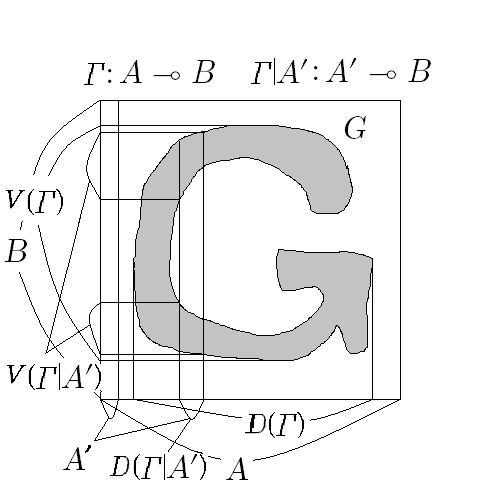
\includegraphics[width=160pt]{1.2.1.a.png}
\end{center}
2つの対応たち$\varGamma:A \multimap B$、$\varDelta:A \multimap B$が与えられたとき、これらの対応たちが等しいかどうかの判定法として、定理\ref{1.2.1.17}が知られており、$\forall a \in A$に対し、$\varGamma\left( \left\{ a \right\} \right) = \varDelta\left( \left\{ a \right\} \right)$が成り立つならそのときに限り、$\varGamma:A \multimap B = \varDelta:A \multimap B$が成り立つことを主張しているのであった。
\begin{thm}
\label{1.2.2.6}
次のことが成り立つ。
\begin{itemize}
\item
  2つの集合たち$A$、$B$の直積$A \times B$とこれの部分集合$G$が与えられれば、対応$\varGamma:A \multimap B = (A \times B,G)$が一意的に決まる。
\item
  1つの対応$\varGamma:A \multimap B$について$A'\in \mathfrak{P}(A)$なる集合$A'$を用いて$V\left( \varGamma|A' \right) = \bigcup_{a \in A'} {V\left( \varGamma|\left\{ a \right\} \right)}$が成り立つ。
\end{itemize}
\end{thm}
\begin{proof}
2つの集合たち$A$、$B$の直積$A \times B$とこれの部分集合$G$が与えられたとき、直積$A \times B$は一意的に存在するかつ、集合$\left\{ \left\{ A \times B \right\},\left\{ A \times B,G \right\} \right\}$も一意的に存在するので、順序対$(A \times B,G)$も一意的に存在する。対応の定義より、よって、対応$\varGamma:A \multimap B = (A \times B,G)$が一意的に決まる。\par
1つの対応$\varGamma:A \multimap B$について$A'\in \mathfrak{P}(A)$なる集合$A'$を用いて次のようになる。
\begin{align*}
V\left( \varGamma|A' \right) &= \left\{ b \in B \middle| \exists a \in A'\left[ (a,b) \in G \right] \right\}\\
&= \bigcup_{a \in A'} \left\{ b \in B \middle| (a,b) \in G \right\}\\
&= \bigcup_{a \in A'} \left\{ b \in B \middle| \exists a \in \left\{ a \right\}\left[ (a,b) \in G \right] \right\}\\
&= \bigcup_{a \in A'} {V\left( \varGamma\left| \text{\{}a \right\} \right)}
\end{align*}
\end{proof}
対応$\varGamma:A \multimap B = (A \times B,G)$において、$\forall(a,b) \in A \times B$に対し、$(a,b) \in G \Leftrightarrow (b,a) \in H$となるような対応$(B \times A,H)$も考えられることができ、これをその対応$\varGamma:A \multimap B$の逆対応といい$\varGamma^{- 1}:B \multimap A$と書くのであった。ここで、その対応$\varGamma^{- 1}$によるその集合$B$の部分集合$B'$の像$V\left( \varGamma^{- 1}|B' \right)$をその対応$\varGamma$によるその集合$B'$の原像、逆像などという。\par
対応$\varGamma:A \multimap B = (A \times B,G)$の逆対応$\varGamma^{- 1}$が$\varGamma^{- 1}:B \multimap A = (B \times A,H)$と与えられたとき、これのgraph$H$については定理\ref{1.2.1.18}より$H = \left\{ (b,a) \in B \times A \middle| (a,b) \in G \right\}$が成り立つのであった。
\begin{thm}
\label{1.2.2.7}
対応$\varGamma:A \multimap B = (A \times B,G)$において、次式たちが成り立つ。
\begin{align*}
\left( \varGamma^{- 1} \right)^{- 1} &= \varGamma\\
D\left( \varGamma^{- 1} \right) &= V(\varGamma)\\
V\left( \varGamma^{- 1} \right) &= D(\varGamma)\\
\left( \varGamma^{- 1} \right)^{- 1}:A \multimap B &= (A \times B,G) = \varGamma:A \multimap B
\end{align*}
\end{thm}
\begin{proof}
対応$\varGamma:A \multimap B = (A \times B,G)$において、これの逆対応$\varGamma^{-1} $のgraphを$H$、これの逆対応$\left( \varGamma^{-1} \right)^{-1} $のgraphを$I$とおくと、$\forall (a,b) \in A\times B$に対し、定理\ref{1.2.1.18}より次のようになることから、
\begin{align*}
(a,b)\in G \Leftrightarrow (a,b) \in H \Leftrightarrow (a,b) \in I
\end{align*}
外延性の公理より$G=I$が成り立ち、対応の定義よりよって、$\left( \varGamma^{- 1} \right)^{- 1} = \varGamma$が成り立つ。\par
$\forall b \in D\left( \varGamma^{- 1} \right)$に対し、次のようになる。
\begin{align*}
b \in D\left( \varGamma^{- 1} \right) &\Leftrightarrow b \in \left\{ b \in B \middle| V\left( \varGamma^{- 1} \right) \neq \emptyset \right\}\\
&\Leftrightarrow b \in B \land V\left( \varGamma^{- 1} \right) \neq \emptyset\\
&\Leftrightarrow b \in B \land \neg\left( \left\{ a \in A \middle| \exists b \in B\left[ (b,a) \in G' \right] \right\} = \emptyset \right)\\
&\Leftrightarrow b \in B \land \neg\left( \left\{ a \in A \middle| \exists b \in B\left[ (a,b) \in G \right] \right\} = \left\{ a \in A \middle| \bot \right\} \right)
\end{align*}
外延性の公理より$\forall a \in A$に対し、次のようになる。
\begin{align*}
&\quad \left( a \in \left\{ a \in A \middle| \exists b \in B\left[ (a,b) \in G \right] \right\} \Leftrightarrow a \in \left\{ a \in A \middle| \bot \right\} \right)\\
&\Leftrightarrow \left( a \in A \land \exists b \in B\left[ (a,b) \in G \right] \Leftrightarrow a \in A \land \bot \right)\\
&\Leftrightarrow \left( a \in A \land \exists b \in B\left[ (a,b) \in G \right] \Leftrightarrow \bot \right)\\
&\Leftrightarrow \neg\left( \left( a \in A \land \exists b \in B\left[ (a,b) \in G \right] \right) \vee \bot \right) \\
&\quad \vee \left( a \in A \land \exists b \in B\left[ (a,b) \in G \right] \land \bot \right)\\
&\Leftrightarrow \neg\left( a \in A \land \exists b \in B\left[ (a,b) \in G \right] \right) \vee \bot\\
&\Leftrightarrow \neg\left( a \in A \land \exists b \in B\left[ (a,b) \in G \right] \right)
\end{align*}
以上より、次のようになる。
\begin{align*}
b \in D\left( \varGamma^{- 1} \right) &\Leftrightarrow b \in B \land \neg\forall a \in A\left[ \neg\left( a \in A \land \exists b \in B\left[ (a,b) \in G \right] \right) \right]\\
&\Leftrightarrow b \in B \land \exists a \in A\left[ a \in A \land \exists b \in B\left[ (a,b) \in G \right] \right]\\
&\Leftrightarrow b \in B \land \exists a \in A\exists b \in B\left[ (a,b) \in G \right]\\
&\Leftrightarrow \exists b \in B\left[ b \in B \land \exists a \in A\left[ (a,b) \in G \right] \right]\\
&\Leftrightarrow \exists b \in B\exists a \in A\left[ (a,b) \in G \right]\\
&\Leftrightarrow b \in B \land \exists a \in A\left[ (a,b) \in G \right]\\
&\Leftrightarrow b \in \left\{ b \in B \middle| \exists a \in A\left[ (a,b) \in G \right] \right\}\\
&\Leftrightarrow b \in V(\varGamma)
\end{align*}
外延性の公理より、よって、$D\left( \varGamma^{- 1} \right) = V(\varGamma)$が成り立つ。\par
$\left( \varGamma^{- 1} \right)^{- 1} = \varGamma$と$D\left( \varGamma^{- 1} \right) = V(\varGamma)$が成り立つのであったので、$D\left( \left( \varGamma^{- 1} \right)^{- 1} \right) = V\left( \varGamma^{- 1} \right)$も成り立つ。よって、$V\left( \varGamma^{- 1} \right) = D(\varGamma)$が成り立つ。
\end{proof}
%\hypertarget{ux5199ux50cf}{%
\subsubsection{写像}%\label{ux5199ux50cf}}
対応$f:A \multimap B$について、$\forall a \in A\exists b \in B$に対し、$V\left( f|\left\{ a \right\} \right) = \left\{ b \right\}$が成り立つとき、その対応$f$を写像といい$f:A \rightarrow B$、$A\overset{f}{\rightarrow}B$などと書く。この写像$f:A \rightarrow B$全体の集合を$\mathfrak{F}(A,B)$、$B^{A}$などと書く。このとき、$V\left( f|\left\{ a \right\} \right) = \left\{ b \right\}$のことを、単に、$f(a) = b$と書き、これを明示するとき、その写像$f$を$f:A \rightarrow B;a \mapsto f(a) = b$などと書くときがありその元$b$をその元$a$のその写像$f$による像、その元$a$におけるその写像$f$の値などといいこのことをその写像$f$はその元$a$をその元$b$に写す、その元$a$にその元$b$を対応させるなどという。\par
これらの用語たちは次の図のように該当される。
\begin{center}
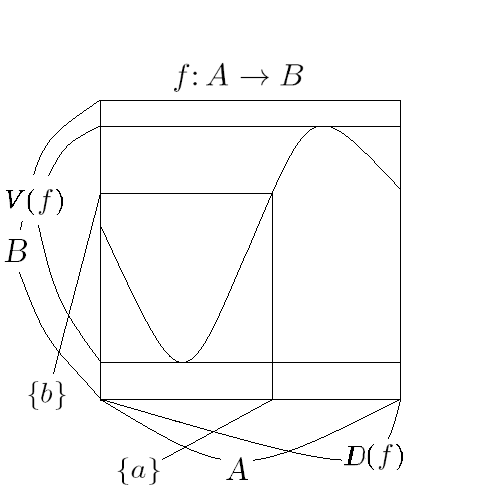
\includegraphics[width=160pt]{1.2.1.b.png}
\end{center}
\begin{thm}
\label{1.2.2.8}
対応$\varGamma:A \multimap B$と写像$f:A \rightarrow B$について、$A',A''\in \mathfrak{P}(A)$、$B',B''\in \mathfrak{P}(B)$なる集合たち$A'$、$A''$、$B'$、$B''$を用いると、次式が成り立つ。
\begin{align*}
A' \subseteq A'' &\Rightarrow V\left( \varGamma|A' \right) \subseteq V\left( \varGamma|A'' \right)\\
V\left( \varGamma|A' \cup A'' \right) &= V\left( \varGamma|A' \right) \cup V\left( \varGamma|A'' \right)\\
V\left( \varGamma|A' \cap A'' \right) &\subseteq V\left( \varGamma|A' \right) \cap V\left( \varGamma|A'' \right)\\
V\left( f^{- 1}|B' \cap B'' \right) &= V\left( f^{- 1}|B' \right) \cap V\left( f^{- 1}|B'' \right)\\
V\left( \varGamma|A \setminus A' \right) &\supseteq V\left( \varGamma|A \right) \setminus V\left( \varGamma|A' \right)\\
V\left( f^{- 1}|B \setminus B' \right) &= A \setminus V\left( f^{- 1}|B' \right)\\
V\left( f^{- 1}|V\left( f|A' \right) \right) &\supseteq A'\\
V\left( f|V\left( f^{- 1}|B' \right) \right) &\subseteq B'
\end{align*}
\end{thm}
\begin{proof}
対応$\varGamma:A \multimap B$について、$A',A''\in \mathfrak{P}(A)$、$B',B''\in \mathfrak{P}(B)$なる集合たち$A'$、$A''$、$B'$、$B''$を用いその対応$\varGamma$のgraphを$G$、これの逆対応のgraphを$G'$、その集合$A$の元の1つを$\overline{a}$、その集合$B$の元々2つを$\overline{b}$、$\overline{\overline{b}}$とする。このとき、$A' \subseteq A''$が成り立つなら、次のようになる。
\begin{align*}
b \in V\left( \varGamma|A' \right) &\Leftrightarrow b \in B \land \exists a \in A'\left[ (a,b) \in G \right]\\
&\Leftrightarrow b \in B \land \exists a \in A' \subseteq A''\left[ (a,b) \in G \right]\\
&\Rightarrow b \in B \land \exists a \in A''\left[ (a,b) \in G \right] \\
&\Leftrightarrow b \in V\left( \varGamma|A'' \right)
\end{align*}
したがって、$V\left( \varGamma|A' \right) \subseteq V\left( \varGamma|A'' \right)$が成り立ち、よって、次式が成り立つ。
\begin{align*}
A' \subseteq A'' \Rightarrow V\left( \varGamma|A' \right) \subseteq V\left( \varGamma|A'' \right)
\end{align*}\par
また、次のようになる。
\begin{align*}
b \in V\left( \varGamma|A' \cup A'' \right) &\Leftrightarrow b \in B \land \exists a \in A' \cup A''\left[ (a,b) \in G \right]\\
&\Leftrightarrow b \in B \land \overline{a} \in A' \cup A'' \land \left( \overline{a},b \right) \in G\\
&\Leftrightarrow b \in B \land \left( \overline{a} \in A' \vee \overline{a} \in A'' \right) \land \left( \overline{a},b \right) \in G\\
&\Leftrightarrow \left( b \in B \land \overline{a} \in A' \land \left( \overline{a},b \right) \in G \right) \\
&\quad \vee \left( b \in B \land \overline{a} \in A' \land \left( \overline{a},b \right) \in G \right)\\
&\Leftrightarrow \left( b \in B \land \exists a \in A'\left[ (a,b) \in G \right] \right) \\ 
&\quad \vee \left( b \in B \land \exists a \in A''\left[ (a,b) \in G \right] \right)\\
&\Leftrightarrow b \in V\left( \varGamma|A' \right) \vee b \in V\left( \varGamma|A'' \right) \\
&\Leftrightarrow b \in V\left( \varGamma|A' \right) \cup V\left( \varGamma|A'' \right)
\end{align*}
よって、次式が成り立つ。
\begin{align*}
V\left( \varGamma|A' \cup A'' \right) = V\left( \varGamma|A' \right) \cup V\left( \varGamma|A'' \right)
\end{align*}\par
また、次のようになる。
\begin{align*}
b \in V\left( \varGamma|A' \cap A'' \right) &\Leftrightarrow b \in B \land \exists a \in A' \cap A''\left[ (a,b) \in G \right]\\
&\Leftrightarrow b \in B \land \overline{a} \in A' \cap A'' \land \left( \overline{a},b \right) \in G\\
&\Leftrightarrow b \in B \land b \in B \land \overline{a} \in A' \land \overline{a} \in A'' \\
&\quad \land \left( \overline{a},b \right) \in G \land \left( \overline{a},b \right) \in G\\
&\Rightarrow b \in B \land \exists\overline{a} \in A'\left[ \left( \overline{a},b \right) \in G \right] \\
&\quad \land b \in B \land \exists\overline{a} \in A''\left[ \left( \overline{a},b \right) \in G \right]\\
&\Leftrightarrow b \in V\left( \varGamma|A' \right) \land b \in V\left( \varGamma|A'' \right) \\
&\Leftrightarrow b \in V\left( \varGamma|A' \right) \cap V\left( \varGamma|A'' \right)
\end{align*}
よって、次式が成り立つ。
\begin{align*}
V\left( \varGamma|A' \cap A'' \right) \subseteq V\left( \varGamma|A' \right) \cap V\left( \varGamma|A'' \right)
\end{align*}\par
また、次のようになる。
\begin{align*}
a \in V\left( f^{- 1}|B' \right) \cap V\left( f^{- 1}|B'' \right) &\Leftrightarrow a \in V\left( f^{- 1}|B' \right) \land a \in V\left( f^{- 1}|B'' \right)\\
&\Leftrightarrow \left( a \in A \land \exists b \in B'\left[ (a,b) \in G \right] \right) \\
&\quad \land \left( a \in A \land \exists b \in B''\left[ (a,b) \in G \right] \right)\\
&\Leftrightarrow a \in A \land \exists b \in B'\left[ (a,b) \in G \right] \land \exists b \in B''\left[ (a,b) \in G \right]\\
&\Leftrightarrow a \in A \land \overline{b} \in B' \land \left( a,\overline{b} \right) \in G \land \overline{\overline{b}} \in B'' \land \left( a,\overline{\overline{b}} \right) \in G\\
&\Leftrightarrow a \in A \land \overline{b} \in B' \land a \in \left\{ a \right\} \land \left( a,\overline{b} \right) \in G \\
&\quad \land \overline{\overline{b}} \in B'' \land a \in \left\{ a \right\} \land \left( a,\overline{\overline{b}} \right) \in G\\
&\Leftrightarrow a \in A \land \overline{b} \in \left\{ \overline{b} \in B' \middle| \exists a \in \left\{ a \right\}\left[ \left( a,\overline{b} \right) \in G \right] \right\} \\
&\quad \land \overline{\overline{b}} \in \left\{ \overline{\overline{b}} \in B'' \middle| \exists a \in \left\{ a \right\}\left[ \left( a,\overline{\overline{b}} \right) \in G \right] \right\}\\
&\Leftrightarrow \forall a \in A\left[ \overline{b} \in V\left( f|\left\{ a \right\} \right) \subseteq B' \land \overline{\overline{b}} \in V\left( f|\left\{ a \right\} \right) \subseteq B'' \right]
\end{align*}
ここで、その対応$f$は写像なので、$\forall a \in A$に対し、$V\left( f|\left\{ a \right\} \right) = \left\{ b \right\}$が成り立つ。したがって、次のようになる。
\begin{align*}
a \in V\left( f^{- 1}|B' \right) \cap V\left( f^{- 1}|B'' \right) &\Leftrightarrow \forall a \in A\left[ \overline{b} \in \left\{ b \right\} \land \overline{\overline{b}} \in \left\{ b \right\} \right]\\
&\Leftrightarrow \forall a \in A\left[ b = \overline{b} = \overline{\overline{b}} \right]
\end{align*}
これにより、$b = \overline{b} = \overline{\overline{b}}$が成り立つので、次のようになる。
\begin{align*}
a \in V\left( f^{- 1}|B' \right) \cap V\left( f^{- 1}|B'' \right) &\Leftrightarrow a \in A \land \overline{b} \in B' \land \left( a,\overline{b} \right) \in G \land \overline{\overline{b}} \in B'' \land \left( a,\overline{\overline{b}} \right) \in G\\
&\Rightarrow a \in A \land \overline{b} \in B' \land \overline{b} \in B'' \land \left( a,\overline{b} \right) \in G\\
&\Leftrightarrow a \in A \land \overline{b} \in B' \cap B'' \land \left( a,\overline{b} \right) \in G\\
&\Leftrightarrow a \in A \land \exists b \in B' \cap B''\left[ (a,b) \in G \right]\\
&\Leftrightarrow a \in \left\{ a \in A \middle| \exists b \in B' \cap B''\left[ (a,b) \in G \right] \right\}\\
&\Leftrightarrow a \in V\left( f^{- 1}|B' \cap B'' \right)
\end{align*}
これにより、$V\left( f^{- 1}|B' \right) \cap V\left( f^{- 1}|B'' \right) \subseteq V\left( f^{- 1}|B' \cap B'' \right)$が得られた。ここで、上記の議論により$V\left( f^{- 1}|B' \cap B'' \right) \subseteq V\left( f^{- 1}|B' \right) \cap V\left( f^{- 1}|B'' \right)$が成り立つのであったので、次式が成り立つ。
\begin{align*}
V\left( f^{- 1}|B' \cap B'' \right) = V\left( f^{- 1}|B' \right) \cap V\left( f^{- 1}|B'' \right)
\end{align*}\par
また、次のようになる。
\begin{align*}
b \in V\left( \varGamma|A \right) \setminus V\left( \varGamma|A' \right) &\Leftrightarrow b \in V\left( \varGamma|A \setminus A' \cup A' \right) \setminus V\left( \varGamma|A' \right)\\
&\Leftrightarrow b \in \left( V\left( \varGamma|A \setminus A' \right) \cup V\left( \varGamma|A' \right) \right) \setminus V\left( \varGamma|A' \right)\\
&\Leftrightarrow b \in \left( V\left( \varGamma|A \setminus A' \right) \setminus V\left( \varGamma|A' \right) \right) \\
&\quad \cup \left( V\left( \varGamma|A' \right) \setminus V\left( \varGamma|A' \right) \right)\\
&\Leftrightarrow b \in \left( V\left( \varGamma|A \setminus A' \right) \setminus V\left( \varGamma|A' \right) \right) \cup \emptyset\\
&\Leftrightarrow b \in V\left( \varGamma|A \setminus A' \right) \setminus V\left( \varGamma|A' \right)\\
&\Leftrightarrow b \in V\left( \varGamma|A \setminus A' \right) \cap b \notin V\left( \varGamma|A' \right)\\
&\Rightarrow b \in V\left( \varGamma|A \setminus A' \right)
\end{align*}
よって、次式が成り立つ。
\begin{align*}
V\left( \varGamma|A \setminus A' \right) \supseteq V\left( \varGamma|A \right) \setminus V\left( \varGamma|A' \right)
\end{align*}\par
また、明らかに$B \setminus B' \subseteq B$が成り立つので、次のようになる。
\begin{align*}
a \in V\left( f^{- 1}|B \setminus B' \right) &\Leftrightarrow a \in V\left( f^{- 1}|B \cap \left( B \setminus B' \right) \right)\\
&\Leftrightarrow a \in V\left( f^{- 1}|B \right) \cap V\left( f^{- 1}|B \setminus B' \right)\\
&\Leftrightarrow a \in V\left( f^{- 1}|B \right) \land a \in V\left( f^{- 1}|B \setminus B' \right)
\end{align*}
ここで、$a \in V\left( f^{- 1}|B \setminus B' \right) \cap V\left( f^{- 1}|B' \right)$が成り立つと仮定しよう。このとき、次のようになる。
\begin{align*}
a \in V\left( f^{- 1}|B \setminus B' \right) \cap V\left( f^{- 1}|B' \right) &\Leftrightarrow a \in V\left( f^{- 1}|B \setminus B' \right) \land a \in V\left( f^{- 1}|B' \right)\\
&\Leftrightarrow a \in A \land \exists b \in B \setminus B'\left[ (a,b) \in G \right] \land \exists b \in B'\left[ (a,b) \in G \right]\\
&\Leftrightarrow a \in A \land \overline{b} \in B \setminus B' \land \left( a,\overline{b} \right) \in G \land \overline{\overline{b}} \in B' \land \left( a,\overline{\overline{b}} \right) \in G\\
&\Leftrightarrow a \in A \land \overline{b} \in B \setminus B' \land a \in \left\{ a \right\} \land \left( a,\overline{b} \right) \in G \\
&\quad \land \overline{\overline{b}} \in B' \land a \in \left\{ a \right\} \land \left( a,\overline{\overline{b}} \right) \in G\\
&\Leftrightarrow a \in A \land \overline{b} \in \left\{ \overline{b} \in B \setminus B' \middle| \exists a \in \left\{ a \right\}\left[ \left( a,\overline{b} \right) \in G \right] \right\} \\
&\quad \land \overline{\overline{b}} \in \left\{ \overline{\overline{b}} \in B' \middle| \exists a \in \left\{ a \right\}\left[ \left( a,\overline{\overline{b}} \right) \in G \right] \right\}\\
&\Leftrightarrow \forall a \in A\left[ \overline{b} \in V\left( f|\left\{ a \right\} \right) \subseteq B \setminus B' \land \overline{\overline{b}} \in V\left( f|\left\{ a \right\} \right) \subseteq B' \right]
\end{align*}
ここで、その対応$f$は写像なので、$\forall a \in A$に対し、$V\left( f|\left\{ a \right\} \right) = \left\{ b \right\}$が成り立つ。したがって、次のようになる。
\begin{align*}
a \in V\left( f^{- 1}|B \setminus B' \right) \cap V\left( f^{- 1}|B' \right) &\Leftrightarrow \forall a \in A\left[ \overline{b} \in \left\{ b \right\} \land \overline{\overline{b}} \in \left\{ b \right\} \right]\\
&\Leftrightarrow \forall a \in A\left[ b = \overline{b} = \overline{\overline{b}} \right]
\end{align*}
これにより、$b = \overline{b} = \overline{\overline{b}}$が成り立つので、次のようになる。
\begin{align*}
a \in V\left( f^{- 1}|B \setminus B' \right) \cap V\left( f^{- 1}|B' \right) &\Leftrightarrow a \in A \land \overline{b} \in B \setminus B' \land \left( a,\overline{b} \right) \in G \land \overline{\overline{b}} \in B' \land \left( a,\overline{\overline{b}} \right) \in G\\
&\Rightarrow a \in A \land \overline{b} \in B \setminus B' \land \overline{b} \in B' \land \left( a,\overline{b} \right) \in G\\
&\Leftrightarrow a \in A \land \overline{b} \in B \land \overline{b} \notin B' \land \overline{b} \in B' \land \left( a,\overline{b} \right) \in G\\
&\Leftrightarrow a \in A \land \overline{b} \in B \land \bot \land \left( a,\overline{b} \right) \in G \Leftrightarrow \bot
\end{align*}
これは矛盾しているので、$a \in V\left( f^{- 1}|B \setminus B' \right) \cap V\left( f^{- 1}|B' \right)$が成り立たないことになる。したがって、$a \in V\left( f^{- 1}|B \setminus B' \right) \Rightarrow a \notin V\left( f^{- 1}|B' \right)$が成り立つ。\par
これにより、次のようになる。
\begin{align*}
a \in V\left( f^{- 1}|B \setminus B' \right) &\Leftrightarrow a \in V\left( f^{- 1}|B \right) \land a \in V\left( f^{- 1}|B \setminus B' \right)\\
&\Rightarrow a \in V\left( f^{- 1}|B \right) \land a \notin V\left( f^{- 1}|B' \right)\\
&\Leftrightarrow a \in V\left( f^{- 1}|B \right) \setminus V\left( f^{- 1}|B' \right)
\end{align*}\par
また、次のようになることから
\begin{align*}
a \in A' &\Rightarrow a \in A \land f(a) \in V\left( f|A' \right)\\
&\Rightarrow a \in A \land \exists b \in V\left( f|A' \right)\left[ b = f(a) \right]\\
&\Rightarrow a \in V\left( f^{- 1}|V\left( f|A' \right) \right)
\end{align*}
次式が得られる。
\begin{align*}
V\left( f^{- 1}|V\left( f|A' \right) \right) \supseteq A'
\end{align*}\par
また、次のようになることから
\begin{align*}
b \in V\left( f|V\left( f^{- 1}|B' \right) \right) &\Leftrightarrow b \in B \land \exists a \in V\left( f^{- 1}|B' \right)\left[ b = f(a) \right]\\
&\Leftrightarrow b \in B \land \overline{a} \in V\left( f^{- 1}|B' \right) \land f\left( \overline{a} \right) = b\\
&\Leftrightarrow b \in B \land \overline{a} \in A \land \exists b' \in B'\left[ f\left( \overline{a} \right) = b' \right] \land f\left( \overline{a} \right) = b\\
&\Leftrightarrow b \in B \land \overline{a} \in A \land \overline{b'} \in B' \land f\left( \overline{a} \right) = \overline{b'} \land f\left( \overline{a} \right) = b\\
&\Rightarrow b \in B \land \overline{b'} \in B' \land b = \overline{b'} \Rightarrow b \in B'
\end{align*}
次式が得られる。
\begin{align*}
V\left( f|V\left( f^{- 1}|B' \right) \right) \subseteq B'
\end{align*}
\end{proof}
\begin{thm}
\label{1.2.2.9}
対応$\varGamma:A \multimap B$と写像$f:A \rightarrow B$について、$\mathcal{A \in}\mathfrak{P}\left( \mathfrak{P}(A) \right)$なる集合$\mathcal{A}$と$\mathcal{B \in}\mathfrak{P}\left( \mathfrak{P}(B) \right)$なる集合$\mathcal{B}$に対し、次式が成り立つ。
\begin{align*}
V\left( \varGamma|\bigcup_{A \in \mathcal{A}} A \right) &= \bigcup_{A \in \mathcal{A}} {V\left( \varGamma|A \right)}\\
V\left( \varGamma|\bigcap_{A \in \mathcal{A}} A \right) &\subseteq \bigcap_{A \in \mathcal{A}} {V\left( \varGamma|A \right)}\\
V\left( f^{- 1}|\bigcap_{B\in \mathcal{B}} B \right) &= \bigcap_{B\in \mathcal{B}} {V\left( f^{- 1}|B \right)}
\end{align*}
\end{thm}
\begin{proof}
対応$\varGamma:A \multimap B$と写像$f:A \rightarrow B$について、$\mathcal{A}\in \mathfrak{P}\left( \mathfrak{P}(A) \right)$なる集合$\mathcal{A}$と$\mathcal{B}\in \mathfrak{P}\left( \mathfrak{P}(B) \right)$なる集合$\mathcal{B}$が与えられたとする。$\forall a \in V\left( \varGamma|\bigcup_{A \in \mathcal{A}} A \right)$に対し、次のようになる。
\begin{align*}
b \in V\left( \varGamma|\bigcup_{A \in \mathcal{A}} A \right)\bigcup_{A \in \mathcal{A}} {V\left( \varGamma|A \right)} &\Leftrightarrow b \in B \land \exists a \in \bigcup_{A \in \mathcal{A}} A\left[ (a,b) \in G \right]\\
&\Leftrightarrow b \in B \land \overline{a} \in \bigcup_{A \in \mathcal{A}} A \land \left( \overline{a},b \right) \in G\\
&\Leftrightarrow b \in B \land \exists A \in \mathcal{A}\left[ \overline{a} \in A \right] \land \left( \overline{a},b \right) \in G\\
&\Leftrightarrow \exists A \in \mathcal{A}\left[ b \in B \land \overline{a} \in A \land \left( \overline{a},b \right) \in G \right]\\
&\Leftrightarrow \exists A \in \mathcal{A}\left[ b \in B \land \exists a \in A\left[ (a,b) \in G \right] \right]\\
&\Leftrightarrow \exists A \in \mathcal{A}\left[ b \in V\left( \varGamma|A \right) \right] \vee b \in V\left( \varGamma|A'' \right)\\
&\Leftrightarrow b \in \bigcup_{A \in \mathcal{A}} {V\left( \varGamma|A \right)}
\end{align*}
よって、次式が成り立つ。
\begin{align*}
V\left( \varGamma|\bigcup_{A \in \mathcal{A}} A \right) = \bigcup_{A \in \mathcal{A}} {V\left( \varGamma|A \right)}
\end{align*}\par
$\forall a \in V\left( \varGamma|\bigcap_{A \in \mathcal{A}} A \right)$に対し、次のようになる。
\begin{align*}
b \in V\left( \varGamma|\bigcap_{A \in \mathcal{A}} A \right) &\Leftrightarrow b \in B \land \exists a \in \bigcap_{A \in \mathcal{A}} A\left[ (a,b) \in G \right]\\
&\Leftrightarrow b \in B \land \overline{a} \in \bigcap_{A \in \mathcal{A}} A \land \left( \overline{a},b \right) \in G\\
&\Leftrightarrow b \in B \land \forall A \in \mathcal{A}\left[ \overline{a} \in A \right] \land \left( \overline{a},b \right) \in G\\
&\Rightarrow \forall A \in \mathcal{A}\left[ b \in B \land \exists\overline{a} \in A\left[ \left( \overline{a},b \right) \in G \right] \right]\\
&\Leftrightarrow \forall A \in \mathcal{A}\left[ b \in V\left( \varGamma|A' \right) \land b \in V\left( \varGamma|A'' \right) \right]\\
&\Leftrightarrow b \in \bigcap_{A \in \mathcal{A}} {V\left( \varGamma|A \right)}
\end{align*}
よって、次式が成り立つ。
\begin{align*}
V\left( \varGamma|\bigcap_{A \in \mathcal{A}} A \right) \subseteq \bigcap_{A \in \mathcal{A}} {V\left( \varGamma|A \right)}
\end{align*}\par 
$\forall a \in \bigcap_{B\in \mathcal{B}} {V\left( f^{- 1}|B \right)} $に対し、次のようになる。
\begin{align*}
a \in \bigcap_{B\in \mathcal{B}} {V\left( f^{- 1}|B \right)} &\Leftrightarrow \forall B\in \mathcal{B}\left[ a \in V\left( f^{- 1}|B \right) \right]\\
&\Leftrightarrow \forall B\in \mathcal{B}\left[ a \in A \land \exists b \in B\left[ (a,b) \in G \right] \right]\\
&\Leftrightarrow a \in A \land \forall B\in \mathcal{B\exists}b \in B\left[ (a,b) \in G \right]\\
&\Leftrightarrow a \in A \land \forall B\in \mathcal{B}\left[ {\overline{b}}_{B} \in B \land \left( a,{\overline{b}}_{B} \right) \in G \right]\\
&\Leftrightarrow a \in A \land \forall B\in \mathcal{B}\left[ {\overline{b}}_{B} \in B \land a \in \left\{ a \right\} \land \left( a,{\overline{b}}_{B} \right) \in G \right]\\
&\Leftrightarrow a \in A \land \forall B\in \mathcal{B}\left[ {\overline{b}}_{B} \in \left\{ {\overline{b}}_{B} \in B' \middle| \exists a \in \left\{ a \right\}\left[ \left( a,{\overline{b}}_{B} \right) \in G \right] \right\} \right]\\
&\Leftrightarrow \forall a \in A\forall B\in \mathcal{B}\left[ {\overline{b}}_{B} \in V\left( f|\left\{ a \right\} \right) \subseteq B \right]
\end{align*}
ここで、その対応$f$は写像なので、$\forall a \in A$に対し、$V\left( f|\left\{ a \right\} \right) = \left\{ \overline{b} \right\}$が成り立つ。したがって、次のようになる。
\begin{align*}
a \in \bigcap_{B\in \mathcal{B}} {V\left( f^{- 1}|B \right)} &\Leftrightarrow \forall a \in A\forall B\in \mathcal{B}\left[ {\overline{b}}_{B} \in \left\{ \overline{b} \right\} \right]\\
&\Leftrightarrow \forall a \in A\forall B\in \mathcal{B}\left[ \overline{b} = {\overline{b}}_{B} \right]
\end{align*}
これにより、$\forall B\in \mathcal{B}$に対し、$\overline{b} = {\overline{b}}_{B}$が成り立つので、次のようになる。
\begin{align*}
a \in \bigcap_{B\in \mathcal{B}} {V\left( f^{- 1}|B \right)} &\Leftrightarrow \forall a \in A\forall B\in \mathcal{B}\left[ {\overline{b}}_{B} \in V\left( f|\left\{ a \right\} \right) \subseteq B \right]\\
&\Rightarrow \forall a \in A\forall B\in \mathcal{B}\left[ \overline{b} \in V\left( f|\left\{ a \right\} \right) \subseteq B \right]\\
&\Leftrightarrow a \in A \land \forall B\in \mathcal{B}\left[ \overline{b} \in B \land \left( a,\overline{b} \right) \in G \right]\\
&\Leftrightarrow a \in A \land \forall B\in \mathcal{B}\left[ \overline{b} \in B \right] \land \left( a,\overline{b} \right) \in G\\
&\Leftrightarrow a \in A \land \overline{b} \in \bigcap_{B\in \mathcal{B}} B \land \left( a,\overline{b} \right) \in G\\
&\Leftrightarrow a \in A \land \exists b \in \bigcap_{B\in \mathcal{B}} B\left[ (a,b) \in G \right]\\
&\Leftrightarrow a \in \left\{ a \in A \middle| \exists b \in \bigcap_{B\in \mathcal{B}} B\left[ (a,b) \in G \right] \right\}\\
&\Leftrightarrow a \in V\left( f^{- 1}|\bigcap_{B\in \mathcal{B}} B \right)
\end{align*}
これにより、$\bigcap_{B\in \mathcal{B}} {V\left( f^{- 1}|B \right)} \subseteq V\left( f^{- 1}|\bigcap_{B\in \mathcal{B}} B \right)$が得られた。ここで、上記の議論により$V\left( f^{- 1}|\bigcap_{B\in \mathcal{B}} B \right) \subseteq \bigcap_{B\in \mathcal{B}} {V\left( f^{- 1}|B \right)}$が成り立つのであったので、次式が成り立つ。
\begin{align*}
V\left( f^{- 1}|\bigcap_{B\in \mathcal{B}} B \right) = \bigcap_{B\in \mathcal{B}} {V\left( f^{- 1}|B \right)}
\end{align*}
\end{proof}
\begin{thebibliography}{50}
  \bibitem{1}
    Rei Frontier Tech Blog. "ZFC公理系について:その1". Hatena Blog. \url{https://tech-blog.rei-frontier.jp/entry/2017/11/02/102042}, (2021-04-01 20:30 閲覧)
  \bibitem{2}
    Rei Frontier Tech Blog. "ZFC公理系について:その2". Hatena Blog. \url{https://tech-blog.rei-frontier.jp/entry/2017/11/09/100000}, (2021-04-01 20:30 閲覧)
  \bibitem{3}
    Rei Frontier Tech Blog. "ZFC公理系について:その3". Hatena Blog. \url{https://tech-blog.rei-frontier.jp/entry/2017/11/16/100000} (2021-04-01 20:30 閲覧)
  \bibitem{4}
    松坂和夫, 集合・位相入門, 岩波書店, 1968. 新装版第2刷 p1-39 ISBM978-4-00-029871-1
\end{thebibliography}
\end{document}
